\documentclass[a4paper, french, 12pt]{article}  % DŽclare la classe du document.
% Il existe 5 classes sous LaTeX : article, book, report, letter et slides 
% Les options de classe sont entre crochets et permettent de faire des choix d'ordre gŽnŽral :
% - dŽfinir la taille de base des caractres avec 10pt, 11pt, 12pt, les commandes d'agrandissement 
% ou de rŽduction de la tailles des caractres ( \small \large ) se feront alors par rapport ˆ cette base
% - dŽfinir la taille du papier:  a4paper,  a5paper, b5paper, executivepaper, legalpaper ou letterpaper
% Utiliser a4paper ds que la papier utilisŽ est de ce format c'est ˆ dire ... tout le temps ;-)
% - utiliser des options de mise en page : 
%       ->   landscape passe en mode paysage pour l'ensemble du doccument
%       ->   onecolumn  option par dŽfaut, le texte sera sur une seule colonne 
%       ->   twocolumn   pour un doccument sur deux colonnes, des rŽglages sont possibles (cf doc & net)
%       ->   oneside toutes les pages seront traitŽs identiquement, par dŽfaut avec la classe article
%       ->   twoside  mise en page diffŽrentes pour les pages pairs et impairs par dŽfaut avec book
%       ->   openright et openany  pour gŽrer le commencement des chapitres dans la classe book
%       ->   titlepage et notitlepage indique si une nouvelle page doit tre commencŽe aprs le titre du document.

% \usepackage permet de dŽclarer un module qui sera pris en compte dans la suite. 
% Les modules permettent d'Žtendre les fonctionnalitŽ de LaTeX

%%%%Caracteres reserves%%%%%%%%%%%
%Pour les obtenir on les fait précéder d'un \
% { s'obtient avec \{
% } s'obtient avec \}
% % s'obtient avec \%
% $ s'obtient avec \$
% & s'obtient avec \&
% # s'obtient avec \#
% _ s'obtient avec \_
% ^ s'obtient avec \^{}
% \ s'obtient avec \textbackslash{} car \\ est une commande
%Les caractères [ et ] ne sont pas réservés et s'obtiennent directement
%\[ et \] delimitent une environnement mathematique
%%%%%%%%%%%%%%%%%%%%%%%%%%%%%%%%%%%%%%%%%%%


%%%%%Polices%%%
%La police employee par defaut par Latex s'appelle Computer Modern

%%%Changement de style de police%%

%Police par defaut {\normalfont ...} c'est une bascule

%Trois familles 
%Romaine par defaut
%sans serif \textsf{..} ou {\sffamily ....}
%typewriter \texttt{..} ou {\ttfamily ....}

%Quatre formes
%droite par defaut
%italique \textit{..} ou {\itshape ....}
%penchee \textsl{..} ou {\slshape ....}
%petites capitales  \textsc{..} ou {\scshape ....}

%Deux series
%normale par defaut
%grasse \textbf{..} ou {\bfseries ....}


%%Taille%%
%Toutes les commandes suivantes sont des bascules a utiliser entre accolades
%{\tiny petit mot}
%Dans l'ordre croissant
%\tiny
%\scriptsize
%\footnotesize
%\small
%\normalsize
%\large
%\Large
%\LARGE
%\huge
%\Huge

%%%%%%%%%%%%%%%%%%%%%%%%%

%%%%%Justification%%%%%
%Alignement a droite
%\begin{flushright}
%{\raggedleft texte \par} ne pas oublier \par
%\leftline{texte}
%\filleft pour formater un titre 

%Alignement a gauche
%\begin{flushleft}
%{\raggedright texte \par} ne pas oublier \par
%\rightline{texte}
%\filright pour formater un titre 


%Centrage
%\begin{center}
%{\centering texte \par} ne pas oublier \par
%\centerline{texte}
%\filcenter pour formater un titre 
%%%%%%%%%%%%%%%%%%%%%%%%%%%%%%%%%%%%%%%%%%%

%%%%%%Espaces%%%%%%%%%%%%%%%%%%%%%


%%Espaces verticaux%%%
%\vskip 2cm  (argument eventuellement negatif), l'espace est ignore s'il coincide avec un saut de page
%\vspace*{2cm} (argument eventuellement negatif), l'espace n'est pas ignore s'il coincide avec un saut de page
%\vspace{2cm} est synonyme de \vskip 2cm 

%%Espaces horizontaux%%%%

%\hskip equivalent a \vskip
%\hspace{?} et \hspace*{?}
%Le cadratin est un espace horizontal egal a la taille de la police utilisee
%\thinspace espace d'un sixieme de cadratin
%\enskip pour un demi-cadratin
%\quad pour un cdratin
%\qquad pour deux cadratins

%%%%%%%%%%%%%%%%%%%%%%%%%%%%%%%%%%%%

%Le moteur eTeX est aujourd'hui utilisé par toutes les distributions (MikTeX, TeXlive) à la place de l'ancien TeX (en fait, c'est plutôt PDFTeX, le successeur de eTeX, qui est utilisé ; contrairement à ce que son nom indique, il peut produire du dvi). Le fait d'utiliser le moteur eTeX au lieu de TeX donne accès à des choses en plus (par exemple à \middle pour aller avec \left et \right, mais aussi à des commandes bien pratiques comme \numexpr, \dimexpr, \detokenize, etc. ainsi qu'à des ressources supplémentaires, comme plus de compteurs disponibles).

%Lorsqu'on utilise le moteur eTeX, certaines de ces fonctionnalités sont automatiquement accessibles (c'est le cas de \middle, \numexpr, etc.), mais pas d'autres (c'est le cas des compteurs supplémentaires). Pour activer ces fonctionnalités manquantes, on peut charger le package etex.sty. Ainsi, l'utilisation d'etex.sty est une solution courante au problème d'avoir trop de compteurs définis (c'est le cas si on charge ensemble trop de packages du type tikz, pstricks, xymatrix, ...)

\usepackage{etex}

%%%%%%%%%%%%Encodage du fichier source %%%%%%%%%%%
\usepackage[T1]{fontenc}
\usepackage[utf8]{inputenc}


%%%%%%%%%%%%%%%Francisation%%%%%%%%%%%%%%
\usepackage[french]{babel}
\frenchbsetup{StandardLists=true}
%%%%%%%%%%%%%%%%%%%%%%%%%%%%%%%%%%%%%%%%%

%%%%%%%%%%%%Mise en page, Reglages genrraux%%%%%%%

%\title{il n'existe pas de plus grand nombre premier}
%\author[Euclide \thanks{Merci Aristote}}
%\date{12 juin $-260$}  Par défaut Latex insère la date du jour
%puis écrire après \begin{document} la commande \maketitle


\usepackage[a4paper,headheight=35 pt, headsep=15pt,top=20 pt,hmargin=1 cm,bottom=20 pt,includeheadfoot]{geometry}
%\usepackage[a4paper,hmargin=1 cm,bottom=2cm,top=2cm,headheight=15pt]{geometry}      
%top est la marge supérieure entre le haut de body et le bord supérieur de la feuille
% \usepackage[left= 4cm,right = 3cm,top= 2cm, bottom=2cm]{geometry} pour le réglage des marges 
% \usepackage[top= 17mm,textheight=23cm,heightrounded,left=25mm,textwidth=16cm] {geometry} pour fixer la hauteur,  la largeur  du texte. heightrounded, autorise le package à arrondir la hauteur textheight à un nombre entier de lignes pour éviter des problèmes de remplissage vertical underfull vbox 


\usepackage{setspace}  % pour le réglage de l'interligne
%Bascule \doublespacing  ou environnement {doublespace}
%Bascule \onehalfspacing  ou environnement {onehalfspace}
%Bascule \singlespacing  ou environnement {singlespace}
% ou encore \renewcommand{\baselinestretch}{n} ou encore l'environnement spacing{n}

%%Package fullpage
%\usepackage[cm]{fullpage}
%where possible options for fullpage are
%in (default) sets the margins to one inch;
%cm sets the margins to 1.5 cm (one centimeter is really too
%little);
%plain (default) selects the plain page style, i.e., with no head-
%ers but only a footer;
%empty for neither headers nor footers;
%headings for both header and footers;
%myheadings also for both headers and footers.
%For the last 4 options, the corresponding \pagestyle declaration is exe-
%cuted, so that it is not necessary to give it again.


%%Pour la numerotation des bas de pages avec le compteur lastpage%%%
\usepackage{lastpage}

%%%%Pour afficher certaines pages au format paysage%%
\usepackage{lscape}
%\begin{landscape}

%%%Plusieurs colonnes
\usepackage{multicol}
%\begin{multicols}[titre]{nb colonnes}
\setlength{\columnseprule}{0.25pt}


%%%%%Références, Notes de bas de pages ou de marges%%%%%%%%%

%%Pour placer une note de bas de page : commande \footnote{}
%Pour placer une note dans la marge : \marginpar{}
%Pour plcaer une note dans un tableau : appel de note avec \footnotemark{} puis le texte après le tableau avec \footnotetext{texte}

%Etiquette  avec \label{nom} puis référence à l'étiquette (numéro de section le plus proche ) avec \ref{nom} ou à lap age avec \pageref{nom}
\usepackage{varioref}
%Introduit  les commandes \vref{} et \vpageref{} qui améloirent l'affichage ainsi que la commande \vpagerefrange{label1}{label2} pour faire référence à tout un bloc de pages entre deux étiquettes
\usepackage{nameref}


%%%%Présentation des titres de section%%%

%\usepackage[clearempty]{titlesec} problème avec PDFLatex ?

%Pour changer la police des titres de sectionnement, un exemple :
%\titleformat*{\section}{\sffamily}

%Pour modifier la police mais aussi la présentation :
%\titleformat{commande}[shape]{format}{label}{sep}{before}{after}
% commande est la commande de sectionnement comme \section
%shape peut etre hang (défaut),frame (encadre), display( paragraphe séparé), block (paragraphe), runin (dans le texte, wrap (comme wrapfigure), leftmargin ou rightmargin
%format est le formatage du titre complet (numéros inclus)éventuellemnt précédé de commandes à inclure avant le titre
% Ces commandes peuvent etre \titleline[r,c ou l]{texte} ou \titlerule[epaisseur] ou \titlerule*[epaisseur]{texte}
%label est la présentation du numero
%sep est l'espace entre le numero et le titre
%before est le code à exécuter avant le titre de section (numero exclu)
%after est le code à exécuter après (vide en général)

%Pour gérer l'espacement
%\titlespacing{commande}{left}{beforesep}{aftersep}[right]
%left est la marge à gauche, beforesep l'espace vertical avant etc ..


%Exemple de présentation de titre encadé :
%\titleformat{\section}[frame]{\titleline[r]{\rule{2in }{2pt}} \normalfont}{\filright\small\ SECTION \thesection\hfill}{7pt}{\LARGE \bfseries\filcenter}{}
%\section{un titre de section encadre}


%%%%%%%%%%%%%%%%%%%%%%%%%%%%%%%%%%%%%%%%%%%% 

%%%%%%%Réglages de la table des matières%%%%
\usepackage{tocvsec2}
%Définir la progondeur : \setcounter{tocdepth}{1}  :
%1 correspond aux chapitres; 2 aux sections etc ...
%Rédéfinir le nom par défaut  :
%\renewcommand{\contentsname}{Liste des chapitres}
%Modifier une entrée :
%\Chapter[titre court]{titre long}
%Ajouter une entrée :
%\addcontentsline{toc}{section}{Nom de la section qu'on veut ajouter}
%Pour exclure une entrée 
%Utiliser une commande étoilée comme \section*
%Pour ajouter  ce qu'on veut dans la table des matières comme des indications de mise n page :
%\addtocontents{toc}{\protect \pagebreak}


%%%%%%%%%%%% Packages pour le texte %%%%%%%%%%%%
\usepackage{lmodern}       %Joli fonte

\usepackage{pifont,fourier}
\usepackage[normalem]{ulem}
%\uline{} pour  un soulignement simple
%Commmandes \uuline{} pour un soulignement double
%\uwave{} pour un soulignement  avec des vagues
% \sout{} pour barrer et \xout{} pour hachurer
\usepackage{cancel} %Commande \cancel{} pour barrer en oblique
%\usepackage{soul}    %souligner
%\usepackage{lettrine} %Pour commencer un paragraphe avec une lettrine
%Package incompatible avec tabvar.tex
%\lettrine{S}{i vous souhaitez}
%\renewcommand{\LettrineFontHook}{\itshape}
%\renewcommand{\LettrineTextFont}{\sffamily}

%%%Pour des jolis boites%%%
\usepackage{fancybox}  
%Commandes \box{} \ovalbox{} \shadowbox{}
%\cornersize{}2 réglage de l'arrondi
% Dimension à régler avec \setlength{}  : \fboxsep \fboxrule  

%%% Pour faire tourner le texte %%%
\usepackage{rotating}  %\begin{turn}{-60} tourné \end{turn} pour tourner un paragraphe
						%pour tourner un texte, commande \rotatebox[origin=c]{angle}{texte}
						
%%Divers%%%%
\usepackage{eurosym}  %pour le symbole de l'euro

\usepackage{url} %pour la gestion des adresses web avec la commande \url{}

%%%%%%%%%%%

%%%%%%%%%%%%%%%Ecriture d'algorithmes Insertion de code source %%%%%%%%%%%

%%%%%Package verbatim%%%%

\usepackage{verbatim} 
%LE package verbatim améliore la présentation des verbatim
% Il  fournit un environnement {comment} pour insérerer des commentaires
%dans le fichier source sans faire précéder toutes les lignes de %

\usepackage{alltt, moreverb} 
%L'environnement verbatimboxed permet d'encadrer un texte en verbatim
% De plus les caractères spéciaux \ et { ne sont pas désactivés (mais #, $ et % le sont)
% et on peut saisir des formules mathématiques avec \( .. \) ou \[ ... \]

%%Pour améliorer envore la présentation des verbatim%%%%
\usepackage{fancyvrb}


%%Couleur
\usepackage[table]{xcolor}
% options : rgb,cmyk,gray,hsb,html pour transformer automatiquement toutes les couleurs du docuement dans le mode choisi
%\definecolor{mauve}{rgb}{0.7,0,0.43}
%\color{couleur} bascule
%\textcolor{couleur}{texte}
%\pagecolor{couleur}
%\colorbox{couleur}
%\fcolorbox{couleur}




%%%%%%%%%% Nouvelles couleurs
\definecolor{rouge}{rgb}{1,0,0}
\definecolor{bleu}{rgb}{0,0,1}
\definecolor{orange}{rgb}{1.00,0.50,0.00}
\definecolor{vert}{rgb}{0,0.50,0.00}
\definecolor{marron}{rgb}{0.49,0.16,0.06}
\definecolor{mauve}{rgb}{0.42,0.24,0.77}
\definecolor{rpastel}{rgb}{1.00,0.77,0.77}
\definecolor{bpastel}{rgb}{0.70,0.86,0.93}
\definecolor{grisclair}{gray}{0.85}
\definecolor{gristclair}{gray}{0.95}
\definecolor{grisfonce}{gray}{0.4}

%%%%%%%%%%%%%%%%%%¨Puce, Listess%%%%%%%%%%%%%%
\usepackage{enumerate}
\usepackage{enumitem}
%Pour changer la puce de liste dans tout le document :
%AtBeginDocument{\renewcommand{\labelitemi}{\textbullet}}
%%%%%%%%Réglages spécifiques au document%%%%%%%%%

%\setenumerate[1]{label=\textbf{Q\arabic*)}}


%%%%%%%%%%%%Graphiques et Dessins%%%%%%%%%%%%%%

\usepackage{graphicx}		
%\rotatebox[origin=x0x1]{angle}{texte} avec xox1 parmi t (top) l (left) r (right) B (ligne de base) et b (bottomm)
%\resizebox{largeur}{hauteur}{texte} pour faire rentrer u nelement encombrant dans une boite					


\usepackage{epic,eepic}   %Capacités graphiques étendues
%\begin{picture}(0,0) permet d'insérer n'importe quoi, n'importe où sans prendre de place (utilie pour annoter une figure en eps)
%Une autre technique est \makebox[0cm][alignement]{texte}
%Exemple:
%\includegraphics[scale=1]{singe.eps}
%\begin{picture}(0,0)
%\put(-27,10){$\sqrt[3]{8}$}
%\end{picture}



%%%%%%%%%%PSTricks%%%%%%%%%%%%

\usepackage{pstricks,pst-plot,pst-text,pst-tree,pst-eps,pst-fill,pst-node,pst-math,pstricks-add,pst-xkey,pst-eucl}


%%%%%%%Tikz%%%%%%%%%%%%%%%
\usepackage{pgf,tikz,tkz-tab}
% Pour les tableaux de signes ou de variations avec tkz-tab voir https://zestedesavoir.com/tutoriels/439/des-tableaux-de-variations-et-de-signes-avec-latex/#1-13389_tikz-un-package-qui-en-a-dans-le-ventre
\usetikzlibrary{arrows}
\usetikzlibrary{shapes.geometric}
\usetikzlibrary{petri}
\usetikzlibrary{decorations}
\usetikzlibrary{arrows}
\usetikzlibrary{math}
 %Variables must be declared in a tikzmath environment but
       % can be used outside
%       \tikzmath{int \n; \n = 508; \x1 = 1; \y1 =1; 
%                   %computations are also possible
%                    \x2 = \x1 + 1; \y2 =\y1 +3; } 


%%%%%%%%%%%%%%%%%%%%%%%%%%%%%%%%%%%%%%%%
%%%%%%%%%%%Commandes Tikz Perso%%%%%%%%%%%%%%%

% Définition des nouvelles options xmin, xmax, ymin, ymax
% Valeurs par défaut : -3, 3, -3, 3
\tikzset{
xmin/.store in=\xmin, xmin/.default=-3, xmin=-3,
xmax/.store in=\xmax, xmax/.default=3, xmax=3,
ymin/.store in=\ymin, ymin/.default=-3, ymin=-3,
ymax/.store in=\ymax, ymax/.default=3, ymax=3,
}
% Commande qui trace la grille entre (xmin,ymin) et (xmax,ymax)
\newcommand {\grille}[2]
{\draw[help lines,black, thick] (\xmin,\ymin) grid[xstep=#1, ystep=#2] (\xmax,\ymax);}
% Commande \axes
\newcommand {\axes} {
\draw[->,very thick] (\xmin,0) -- (\xmax,0);
\draw[->,very thick] (0,\ymin) -- (0,\ymax);
\draw (0.95*\xmax, 0) node[above] {$x$};
\draw (0, 0.95*\ymax) node[left] {$y$};
}
% Commande qui limite l?affichage à (xmin,ymin) et (xmax,ymax)
\newcommand {\fenetre}
{\clip (\xmin,\ymin) rectangle (\xmax,\ymax);}

%Exemple d'utilisation

%\begin{center}
%\begin{tikzpicture} [xmin=-2,xmax=2,ymin=0,ymax=5]
%\grille{1} \axes \fenetre
%\draw plot[smooth] (\x,\x^2);
%\end{tikzpicture}
%\end{center}

%style pour la perspective cavalière française
%voir Tikz pour l'impatient page 68
\tikzset{math3d/.style=
{x= {(-0.353cm,-0.353cm)}, z={(0cm,1cm)},y={(1cm,0cm)}}}

%%%%%%%Symbole pour code calculatrice%%%%%%

%Flèche remplie pour défilement de menu

\newcommand{\flechefillright}{
\begin{tikzpicture}[scale=0.15] \fill (0,0)--(2,1)--(0,2)--cycle;
\end{tikzpicture}}

%%%%%%%%%%%%%Symboles pour calculatrice Casio%%%%
\newcommand{\execasio}{\Pisymbol{psy}{191}} %Retour chariot
\newcommand{\dispcasio}{\begin{pspicture}(.1,.1)\pspolygon*(.1,0)(.1,.1)\end{pspicture}} %Triangle « Disp »
\newcommand{\dispcasiotikz}{\begin{tikzpicture}[scale=0.2]
\fill (0,0) -- (1,0) -- (1,1) -- cycle;
\end{tikzpicture}} %Triangle « Disp »
%

%Fleche entre deux lignes, d'apres 'un bon petit' : http://forum.mathematex.net/latex-f6/fleches-entre-deux-lignes-pour-resolution-d-equation-t10283.html#p99817
\newcommand\addnode[1]{\Rnode{#1}{}}
\newcommand\linknode[3]{\ncbar[angleA=0,angleB=0,nodesep=1ex,arm=10ex,offset=-2pt]{->}{#1}{#2}\Aput{\vphantom{x}#3}}

%%%%%%%%%%%%%%%%%%%%%%%%%%%%%%%%%%%%%%%%
%%%%%%%%%%%Fin Commandes Tikz%%%%%%%%%%%%%%%


%%%%%%%%%%%%Specifiques%%%%%%%%%%%
\usepackage{wrapfig}
%pour insérer une figure à droite ou à gauche d'un texte
%\begin{wrapfigure}[nb lignes]{placement l,r,c,i(inside),o(outside)}[overhang]{width}
%ce package fonctionne mal à proximité des listes
%%%%%%%%%%%%%%%%%%%%%%%%%%%%%%%%%%%%%

%%%%%Environnements et symboles spéciaux pour faire joli%%%%%%

%%%Pour des environnements + jolis avec insertion de logo%%%%
\usepackage{xkeyval}  %indispensable pour bclogo
\usepackage[tikz]{bclogo}

\usepackage{framed}  %Le package « framed» Crée 3 nouveaux environnements, qui se comportent comme des minipage de largeur \linewidth, mais permettant en plus de se casser entre plusieurs pages.     * framed : avec un cadre autour;     * shaded : avec un fonc coloré (il faut définir la couleur shadecolor);     * leftbar : avec une barre le long du côté gauche.

%%%%%%%%%%%%%%%%%%%%%%%%%%%%%%%%%%%


%%%%%%Environnements et symbomles mathématiques%%%%

%%%Tableaux de variations %%%%%%%%%%

\usepackage{variations}

%%%%%%%%%%%AmsMaths%%%%%%
\usepackage{mathtools}        %Commandes essentielles, extension d'amsmath
\usepackage{amsfonts,amssymb}  %Principaux symboles
\usepackage{mathrsfs} %Polices calligraphiques
\usepackage{stmaryrd} %Pour les intervalles d'entiers avec \llbracket et \rrbracket
\usepackage[autolanguage, np]{numprint}
%%%%%%%%%%%%Là encore il y a de grosses différences entre le monde anglo-saxon et les francophones.Le séparateur des décimales est un point en anglais et une virgule en français. Leséparateur des milliers est une virgule en anglais et une espace insécable en français. Ilest préférable d’utiliser le package numprint (\usepackage{numprint}) qui associé àfrenchb produira la bonne typographie.
%123456789 = 123456789 \numprint{123456789} = 123 456 789  \numprint{3,1415926535897932384626} = 3,141 592 653 589 793 238 462 6  \numprint{12.34} = 12,34  En plus tu peux préciser les unités de cette façon : \numprint[kg]{12.34} = 12,34 kg ou encore \numprint[\degres C]{22} = 22°C Si tu veux utiliser le raccourci \np{} au lieu de \numprint{}, il te faut charger le package de cette façon : \usepackage[np]{numprint}
\usepackage[thmmarks,amsmath]{ntheorem}
%Pour définir un nouveau théorème :
%\newtheorem{conj}{Conjecture}[chapter] environnement con d'en tete Conjecture avec numérotation au sein d'un chapitre
%Pour rédéfinir le style d'un théorème, placer les commandes avant \newtheorem et entourer le tout d'accolades
%\theoremstyle{style} : :
% plain est le style par défaut
% break insère un saut de ligne après le titre du théorème
%margin et marginbreak sont les équivalents avec numéro dans la marge
%\theorembodyfont{\normalfont \sffamily} police du corps du théorème
%\theoremheaderfont{\scshape} police de l'en-tete (définie 1 fois pour tous les théorèmes)
%\theoremsymbol{ } symbole ajouté à la fin du théorème
%\theoremseparator{--} élément situé entre le numéro et le corps du theoreme
%\theoremprework{\rule{\linewidth}{0.4pt}} élément précédant chaque théoreme
%\theorempostwork{\dingline{71}} élément suivant chaque théoreme
%\theoremnumbering{Roman} style de numérotation
\usepackage{bbm, dsfont}   %Fonction indicatrice
\usepackage{esint,esvect}  %Flèches supplémentaires.
\usepackage{lcg}  %%%%%%%générer des nombres pseudo aléatoires%%%%


%%%%%%%%%%%Tableaux%%%%%%%%%%%
\usepackage{array}
%\usepackage{multirow} %problème redéfinit la commande \multirow{nligne}*{texte}
\usepackage{tabularx}        % Largeur totale donnée          
\usepackage{longtable}       %Sur plusieurs pages
%\usepackage{diagbox}  %Successeur de slashbox, voir Latex pour l'impatient p. 73, charge pict2e qui redefinit \arc
\usepackage{alterqcm} 
%%%Une commande de David Robert%%%%%%%
%\newcommand{\delair}[1]{\ensuremath\displaystyle\psframebox[framesep=0.15em,linestyle=none]{ \displaystyle#1}}
\newcommand{\delair}[1]{\setlength{\fboxrule}{0mm} \fbox{#1}}
%%%%%%%%%%%%%%%%%%%%%%%%%%%%%%%%%%%%%%




%%%%%%%%%%%%%%Programmation en Latex, Création de nouvelles Commandes%%%%%%%%%%%%%
\usepackage{xspace} %pour la gestion fine des espaces avec la commande \xspace
\usepackage{calc} %   pour faire des calculs avec les longueurs par exemple%%
%Commande \real{0.72} pour le reel 0,72
%\ratio{3}{4} pour le reel 0,75

\usepackage{ifthen}
%Syntaxe d'un test conditionnel : \ifthenelse{condition}{action si realisee}{action sinon}
%Commandes de test :
%\isodd{entier}
%\equal{chaine 1}{chaine 2}
%\lengthtest{comparaison entre deux longueurs} retourne un booleen
%\or, \and, \not \( et \) permettent de combiner des tests avec parenthesages
%
\usepackage{multido}  % package pour utiliser de boucles iteratives

%%%%Boucle Pour%%%

% Sa syntaxe est la suivante : 
% \multido{variables}{nbiteration}{code}
% Le code sera ainsi repete nbiteration fois. Les declarations de variables sont separees par des virgules. Un declaration prend la forme :
%    variable = valeurinitiale + increment  Exemple :
% \multido{\i=0+1}{21}{instruction a repeter } 
%Les variables d'initialisation commencent par i s'il s'agit d'entier, par r s'il s'agit de reels et par d sis ce sont des longueurs
%Exemple de calcul des multiples de pi et d'affichage un par ligne :
%\newcommand{\multipledepi}[1]{\multido{\ia=2+1,\rpi=6.28318530+3.14159265}{#1}{$\ia\pi\approx\rpi$\endgraf}
%Noter que la commande \endgraf synonyme de \par est bien prtique dans les commandes ou \par est interdite

%%%%%Boucle Tant Que%%
%Syntaxe : \whiledo{test}{instruction}
%Exemple d'affichage de lignes pointillees pour laisser la place dans un enonce de controle avec \reponses{7} par exmeple (on peut aussi utilsier \multido dans ce cas)
%\newcounter{nombreentier}
%\newcommand{\reponses}[1]{\setcounter{nombreentier}{0}\whiledo{\value{nombreentier}<#1}{\noindent \dotfill \par \stepcounter{nombreentier}}}



%%%%%%%%%%%%%%%%%%%%%%%%%%%%%%%%%%%%%%%%%%%%%%


%%%%%%%%%%%%%%%%%%%%%%%Longueurs%%%%%%%%%%%%%%%%%%%%%%%%%%

%Attention a la syntaxe :
% Si on a une longueur appelle \longueur :
%\rule{0.72\longueur}{1mm} pas de *
%mais \rule{\real{0.72}*\widthof{exemple}}{1mm}

%unites de longueur : pt, mm, cm ect
%unites qui dependent de la police utilisee : 1 em correspond à l longueur d'un m et 1 ex à la hauteur d'un x
%\setlength{\nom}{valeur}
%\addtolength{\nom}{valeur}
%\settowidth{\nom} \settoheigth{\nom}

%%%%%%Boites avec longueurs caracterisitiques%%%
%\fbox \makebox \framebox utlisent stockent dans \height, \width, \depth, \totalheight les dimensions de l'argument de la commande
%Exemple : \framebox[\width+17mm][positionnement]{un texte encadre}
%DE fçon plus generale on peut acceder aux dimensions d'un objet avec :
%\widthof{texte} \depthof{texte} \heightof{texte}
%Exempel : \rule{\widthof{un exemple}}{1mm}


%%%%%%%%%%%%%%Compteurs%%%%%%
%Un compteur comme celui qui numerote les sections  represente 3 elements distincts  :
%D'abord son nom section
%Ensuiet sa valeur en tant qu'entier : \value{section} (qui vaut 6 dans l'exemple mais qui ne s'affiche pas directment, elle sert d'argument pour d'autres commandes)
%Enfin son apparence \thesection qui affiche par exemple 11.6  pour section 6 du chapitre 11

%Definition d'un nouveau compteur : \newcounter{moncompteur}
%\newcounter{nom}[old] indique que le compteur nom est remis à 0 lorsque le compteur old est a 0
%initialisation : \setcounter{moncompteur}{0}
%ajout d'une valeur : \addtocounter{moncompteur}{valeur} pour ancienne valeur + valeur
%incrementation de 1 : \refstepcounter{moncompteur}
%Pour mieux gerer la remise à 0 d'un compteur en foinction d'un autre compteur :
%\numberwithin{moncompteur}{autrecompteur}

%%%%Redefinition d'un compteur deja existant :
%D'abord on choisit le type de numerotation (\roman \Roman \Arabic \arabic \alpha \Alpha)
\renewcommand{\theenumi}{\textbf{\arabic{enumi}}}
%Puis on choisit l'apparence de l'etiquette
\renewcommand{\labelenumi}{\textbf{\theenumi.}}
\renewcommand{\theenumii}{\textbf{\alph{enumii}}}
\renewcommand{\labelenumii}{\textbf{\theenumii.}}



%%%%%Package à appeler après Babel%%%%%%%%%%%%

%%%%%%%%Flottants%%%%%%%%%%%%%%%%%%%%%%%%
%packages qui doivent etre chargés après le package babel
%car ils utilsient le package caption
\usepackage{float,afterpage}
%Deux types de flottants par défaut : figure et table
%\begin{figure}[préférences de placement dans l'orde de gauche à droite: t,,b,h,p,h!,H]
%\caption[texte court pour la liste]{légende}
%Liste des flottants ; \listoffigures ou \listoftables ou  \listeof{flottant}{titre}
%Placements par défaut pour tout le document: \floatplacement{figure}{t}
%Légende avec \caption{Légende} suivie de \label{Etiquette}
%Quand un flottant passe en mode p aucun autre flottant ne peut etre inséré
%tant qu'une page entire de flottants n'a pas été composée
%Pour vider le stocke de flottants on utilise la commande \clearpage
%\clearpage force u nsaut de page et réserve la page suivante aux flottants
% Pour finir la page en cours, utiliser \afterpage{\clearpage} 

%Défintion de nouveaux flottants
%\newfloat{nom}{positionnement}{extension du fichier de liste}[compteur d'appui]
%\newfloat{ex}{hb}{loex}[chapter]
%\floatname{ex}{\textit{Exemple}} nom dans la légende du flottant
%\floatstyle{boxed}
%\listof{ex}{Liste des exemples de code}

\usepackage[section]{placeins}
%pour que les flottants soient bien inclus dans la section à laquelle ils appartiennent

\usepackage{subfig}
%sous-flottants
%\subfloat[légende]{sous-flottant}
%Pour faire apparaitre les sous-flottants dans la liste des flottants :
%\setcounter{lofdepth}{2}

\usepackage{caption}  %Pour les légendes
%voir Latex pour l'impatient page 94 (pour la commande \captioof{type de flottant}[texte court] {texte}
%voir Latex pour l'impatient page 94 pour le paramétrage  des options de légendes

%%%%%%%%%%%%%%%%%%%Présentation de codes sources%%%%%%%%%%%%%%%%%
\usepackage{listings}
%On utilise l?environnement lstlisting pour insérer
%un code source.
%En plus de l?environnement lstlisting, on peut également utiliser la
%commande \lstinline qui fonctionne comme la commande \verb, en ce
%sens qu?on peut utiliser n?importe quel caractère comme délimiteur. Enfin,
%la commande \lstinputlisting permet de charger un code source depuis
%un fichier externe.
%Il y a deux manières de préciser des options : soit via l?option de l?envi-
%ronnement ou de la commande, soit en utilisant la commande \lstset
%qui permet de définir des options de manière globale.

\lstset{ %
  language=Python,                % the language of the code
  basicstyle=\ttfamily,           % the size of the fonts that are used for the code
  %numbers=left,                   % where to put the line-numbers
  numberstyle=\tiny,  % the style that is used for the line-numbers
  %stepnumber=2,                   % the step between two line-numbers. If it's 1, each line 
                                  % will be numbered
  %numbersep=5pt,                  % how far the line-numbers are from the code
  backgroundcolor=\color{white},      % choose the background color. You must add \usepackage{color}
  showspaces=false,               % show spaces adding particular underscores
  showstringspaces=false,         % underline spaces within strings
  showtabs=false,                 % show tabs within strings adding particular underscores
  frame=single,                   % adds a frame around the code
  rulecolor=\color{black},        % if not set, the frame-color may be changed on line-breaks within not-black text (e.g. comments (green here))
  tabsize=4,                      % sets default tabsize to 2 spaces
  captionpos=b,                   % sets the caption-position to bottom
  breaklines=true,                % sets automatic line breaking
  breakatwhitespace=false,        % sets if automatic breaks should only happen at whitespace
  %title=\lstname,                   % show the filename of files included with \lstinputlisting;
                                  % also try caption instead of title
  breakindent=1cm,
  keywordstyle=\color{blue},          % keyword style
  commentstyle=\color{red},       % comment style
  %stringstyle=\ttfamily\color{green},         % string literal style
  escapeinside={\%*}{*)},            % if you want to add LaTeX within your code
  morekeywords={*,...},              % if you want to add more keywords to the set
  deletekeywords={...}              % if you want to delete keywords from the given language
  upquote=true,columns=flexible,
xleftmargin=1cm,xrightmargin=1cm,
 inputencoding=utf8,			%Les lignes qui suivent sont pour le codage utf8
  extendedchars=true,
  literate=%
            {é}{{\'{e}}}1
            {è}{{\`{e}}}1
            {ê}{{\^{e}}}1
            {ë}{{\¨{e}}}1
            {û}{{\^{u}}}1
            {ù}{{\`{u}}}1
            {â}{{\^{a}}}1
            {à}{{\`{a} }}1
            {î}{{\^{i}}}1
            {ô}{{\^{o}}}1
            {ç}{{\c{c}}}1
            {Ç}{{\c{C}}}1
            {É}{{\'{E}}}1
            {Ê}{{\^{E}}}1
            {À}{{\`{A}}}1
            {Â}{{\^{A}}}1
            {Î}{{\^{I}}}1
}

\lstdefinestyle{rond}{
  numbers=none,
  backgroundcolor=\color{gristclair},
  frameround =tttt
}

\lstdefinestyle{compil}{
  numbers=none,
  backgroundcolor=\color{gristclair}
}
%\lstset{language=Python,basicstyle=\small , frame=single,tabsize=4,showspaces=false,showtabs=false,showstringspaces=false,numbers=left,numberstyle=\tiny , extendedchars=true}



%%%%%%%%%%%Packages spécifiques pour les sorties pdf%%%%%%%%

%%%%Insertion de liens hypertextes %%%%

\usepackage[urlcolor=red,% Liens vers une page web
            linkcolor=blue, %Liens internes au document
            colorlinks=true]{hyperref}


%%%%%   Insertion de pages de fichiers pdf%%%%

\usepackage{pdfpages}

%Le package pdfpages permet d?effectuer facilement des opérations sur
% des fichiers PDF. La première chose qu?on peut faire consiste à insérer
% A certaines pages d?un document PDF dans un document L TEX. On uti- lise pour cela la commande \includepdf. On spécifie les pages que l?on souhaite insérer avec la possibilité de définir des intervalles ou d?insérer une page blanche avec {}, avec l?option pages. L?exemple suivant insère la page 1, suivie d?une page blanche, suivie des pages 5 à 9, suivies de la page 15 du document monDocument.pdf. \includepdf[pages={1,{},5-9,15}]{monDocument.pdf} Il est également possible d?obtenir plusieurs pages par feuille. On utilise pour cela l?option nup. On définit ensuite l?espacement à mettre entre les pages logique avec l?option delta et on peut avoir une bordure autour des pages logiques avec l?option frame. Par exemple, pour insérer toutes les pages du document monDocument.pdf, avec 3 × 2 pages par feuille, séparées par 5mm et une bordure, il faut écrire : \includepdf[pages=-,nup=3x2,frame]{monDocument.pdf} 



%%%%%%%%%%%%%%%%%%%%%%%%%%%%%%%%%%%%%%%%%%%%%%%%%%%%%%%%%%%%
%%%%%%%%%%%%%%%%%%%%%Environnements et commandes persos%%%%%

%%%%%%%Creer son propre fichier de style%%%%
%on regroupe ses commandes dans un fichier d'extension .sty comme local.sty
%%on charge son fichier de style avant le \begin{document} avec \input{local.sty}


%%%%%%%%%%%%%%%%%%%%%%%%%%%%%%%%%%%%%%%%%%%%%%%%%%%%%%%%%%%%%%%%%%%%%%%%
%%%%%%%%%%%%%%%%%%%%Environnements persos%%%%%%%%%%%%%%%%%%%%%%%%%%%%%%%%
%Syntaxe :
%\newenvironment{nom}[nombre d'args][defaut]{definitions initiales}{definitions finales}
%definitions intiales sont les commandes appelées par \begin{nom}
%Definitions finales sont les commandes appelées par \end{nom}

%%%%%%%%%%%%%%%%Définitions des environnemts persostheoreme, exemple ..%%%%
%%%% Exercice avec encadré %%%%
\newcounter{exo}
\newenvironment{exercice}[1]
{\par \bigskip  \noindent \addtocounter{exo}{1} \shadowbox{\textbf{Exercice} \textbf{\theexo}} \hspace{0.5cm}{\itshape #1} \vspace*{10pt} \par}
{\par \bigskip }

%%Sans Numéro
\newenvironment{exerciceStar}[1]
{\par \bigskip  \noindent \addtocounter{exostar}{1} \shadowbox{\textbf{Exercice}} \hspace{0.5cm}{\itshape #1} \vspace*{10pt} \par}
{\par \bigskip }

%%%% Exercice avec trait %%%%
\newcounter{exoB}
\newenvironment{exerciceB}[1]
{\par \bigskip  \noindent \addtocounter{exoB}{1} \hrulefill \quad { \large \textbf{Exercice \theexoB}  {\quad \itshape #1}  } \quad \hrulefill \par \medskip }
{\par \bigskip }


%%Sans option
\newenvironment{exerciceB2}
{\par \bigskip  \noindent \addtocounter{exoB}{1} \hrulefill \quad { \large \textbf{Exercice \theexoB}} \quad \hrulefill \par \medskip }
{\par \bigskip }


%%Sans numéro
\newenvironment{exerciceBStar}[1]
{\par \bigskip  \noindent \hrulefill \quad { \large \bfseries  #1  } \quad \hrulefill \par \medskip}
{\par \bigskip }

%%%% Exercice avec dingbat %%%%

\newcounter{exoC}
\newenvironment{exerciceC}[2][101]
{\par \bigskip  \noindent \addtocounter{exoC}{1} \dingfill{#1} {\quad  \large \textbf{Exercice \theexoC} \quad  {\itshape #2} } \dingfill{#1} \par \medskip}
{\par \bigskip }

%%Sans numéro

\newenvironment{exerciceCStar}[2][101]
{\par \bigskip  \noindent \dingfill{#1} \quad {\large \bfseries  #2 } \quad  \dingfill{#1} \par \medskip}
{\par \bigskip }

\newenvironment{cours}[1]
{\par \bigskip  \noindent  \shadowbox{\textbf{Question de cours} } \hspace{0.5cm}{\itshape #1} \vspace*{10pt} \par}
{\par \bigskip }

\newcounter{act}
\newenvironment{activite}[1]
{\par \medskip  \noindent \addtocounter{act}{1} \fbox{\textbf{Activité~} \textbf{\theact}} \hspace{0.5cm}{\itshape #1} \vspace*{10pt} \par}
{\par \bigskip }




\newcounter{blocn}
\newenvironment{blocnote}[1]
{\par \medskip   \addtocounter{blocn}{1} \begin{leftbar} \noindent  \underline{\textbf{Bloc-Note} \textbf{\theblocn}} \hspace{0.5cm}{\itshape #1}   \vspace*{10pt} \par }
{\end{leftbar} \par \bigskip }

\newenvironment{blocnote*}[1]
{\par \medskip    \begin{leftbar} \noindent  \underline{\textbf{Bloc-Note} } \hspace{0.5cm}{\itshape #1}   \vspace*{10pt} \par }
{\end{leftbar} \par \bigskip }

\newenvironment{axiome}[1]
{\par \medskip   \begin{leftbar} \noindent \underline{\textbf{Axiome}}\hspace{0.5cm}{\itshape #1}   \vspace*{10pt} \par }
{\end{leftbar}  \par \medskip }

\newcounter{correc}
\newenvironment{corrige}[1]
{\par \bigskip  \noindent  \addtocounter{correc}{1}\shadowbox{\textbf{Corrigé} \textbf{\thecorrec}} \hspace{0.5cm}{\itshape #1} \vspace*{10pt} \par}
{\par \bigskip }

\newcounter{thme}
\newenvironment{theoreme}[1]
{\par \medskip   \begin{framed} \noindent \addtocounter{thme}{1} \underline{\textbf{Théorème} \textbf{\thethme}} {\itshape #1}  \vspace*{10pt} \par }
{\end{framed} \par \bigskip }

\newcounter{thmedef}
\newenvironment{theoremedef}[1]
{\par \medskip   \begin{framed} \noindent \addtocounter{thmedef}{1} \underline{\textbf{Théorème-Définition} \textbf{\thethmedef}} {\itshape #1}  \vspace*{10pt} \par }
{\end{framed} \par \bigskip }

\newcounter{corollaire}
\newenvironment{corollaire}[1]
{\par \medskip   \begin{framed} \noindent \addtocounter{corollaire}{1} \underline{\textbf{Corollaire} \textbf{\thecorollaire}} {\itshape #1}  \vspace*{10pt} \par }
{\end{framed} \par \bigskip }


\newenvironment{preuve}[1]{ 
\noindent\underline{\textbf{Preuve :}} \hspace{0.5cm}{\itshape #1}\par  \medskip 
\begin{flushleft} \itshape
        }  %instructions initiales de l'environnement
{\hfill$\Box$\end{flushleft}\par \bigskip }  %instructions finales de l'environnement   : symbole de fin de preuve ˆ droite

\newcounter{def}
\newenvironment{definition}
{\par \medskip   \begin{leftbar} \noindent \addtocounter{def}{1}\underline{\textbf{Définition} \textbf{\thedef}}  \vspace*{10pt} \par  }
{\end{leftbar}  \par \medskip }




\newenvironment{methode}[1]
{\par \medskip   \begin{framed} \noindent\underline{\textbf{Méthode}} \hspace{0.5cm}{\itshape #1} \vspace*{10pt} \par  }
{\end{framed} \par \medskip }

\newcounter{rque}
\newenvironment{remarque}
{\par \medskip  \noindent \addtocounter{rque}{1}\underline{\textbf{Remarque} \textbf{\therque}} \itshape \vspace*{10pt} \par}
{\par \medskip }

\newenvironment{remarque*}
{\par \medskip   \noindent\underline{\textbf{Remarque :}}  \\ \noindent}
{\par \medskip }

\newenvironment{definitions}
{\par \medskip   \begin{framed} \noindent \addtocounter{def}{1}\underline{\textbf{Définitions} \textbf{\thedef}} \vspace*{10pt} \par }
{\end{framed} \par \medskip }

\newcounter{prop}
\newenvironment{propriete}[1]
{\par \medskip   \begin{framed} \noindent \addtocounter{prop}{1}
 \underline{\textbf{Propriété} \textbf{\theprop}}\hspace{0.5cm}{\itshape #1}\vspace*{10pt} \par  }
{\end{framed} \par \medskip }

\newcounter{exple}
\newenvironment{exemple}[1]
{\par \medskip  \noindent \addtocounter{exple}{1} \underline{\textbf{Exemple} \textbf{\theexple} } \hspace{0.5cm}{\itshape #1} \vspace*{10pt} \par}
{\par \medskip }

\newenvironment{exemples}
{\par \medskip  \noindent \addtocounter{exple}{1} \underline{\textbf{Exemples} \textbf{\theexple}} \vspace*{10pt} \par}
{\par \medskip }

%Environnement contenu pour un document présentant une progression annuelle
\newenvironment{contenu}
{\par \medskip   \begin {bclogo}[ noborder = true,logo=\bccrayon] \noindent {\large \textbf{Contenu de la séance}} \vspace*{10pt} \par  }
{\end{bclogo}  \par \medskip }

%Environnement programme pour un document présentant une progression annuelle
\newenvironment{programme}
{\par \medskip   \begin {bclogo}[ noborder = true, barre=zigzag,logo=\bcinfo] \noindent {\large \textbf{Programme officiel}} \vspace*{10pt} \par  }
{\end{bclogo}  \par \medskip }

%Environnement programme pour un document présentant une progression annuelle
\newenvironment{ressource}
{\par \medskip   \begin {bclogo}[ noborder = true,logo=\bcbook] \noindent {\large \textbf{Ressources}}\\vspace*{10pt} \par }
{\end{bclogo}  \par \medskip }


\newcounter{alg}
\newenvironment{algorithme}[1]
{\par \medskip   \begin {bclogo}[ noborder = true, barre=zigzag,logo=\bccrayon] \noindent \addtocounter{alg}{1}\underline{\textbf{Algorithme} \textbf{\thealg}} {\itshape #1} \vspace*{10pt} \par  }
{\end{bclogo}  \par \medskip }
%%%%%%%%%%%%%%%%%%%%%%%%%%%%%%%%%%%%%%%%%%%%%%%%


%%%%%%%%%%%%%%%%%%%%%%%%%%%%%%%%%%%%%%%%%%%%%%%%%%%%%%%%%%
%%%%%%%%%%%%%%%%%%%%%%%%%Commandes personnelles%%%%%%%%%%%%%


%%%Syntaxe
%\newcommand{\nom}[nombre d'arguments][valeur par defaut de l'argument optionnel]{definition}
%L'argument optionnel est toujours le premier
%Exemple : \newcommand{\Sf}[2][\bfseries]{{\sffamily#1#2}}
%utilisation : \Sf{texte} avec la valeur par defaut ou \Sf[\itshape]{texte}



%%%%%%%%%%%%%%%%%Commandes  de Pierre Duclosson %%%%%%%%%%%%%%%%%%%%%%%
% ----- DŽfinition de la macro pour le quadrillage des zones laissŽes libres pour les notes des Žlves   

\newcommand{\quadrillage}[1]{
\setlength{\unitlength}{1mm}
\vskip 0,5cm
\multido{\i=0+1}{#1}{%
     \begin{picture}(150,5)
     \linethickness{0,005mm}
     \put(-7,0){\grid(170,5)(5,5)}
     \end{picture}\vskip 0,001cm
     }
\vskip 0,5cm
}

% -------  Une autre macro pour laisser une zone libre blanche de tant de ligne  par exemple \ligne{12}  laisse 12 lignes

\newcommand{\ligne}[1]{%
\vskip 0,5cm   
% si tu veux placer un repre au dŽbut de l'espace libre c'est ici
\multido{\i=0+1}{#1}{%
    \vphantom{X}
    }
% si tu veux placer un repre ˆ la fin de l'espace libre c'est ici
\vskip 0,5cm
}

%  ------  Une macro pour tracer des lignes en pointillŽs dans l'esprit des prŽcŽdentes 

\newcommand{\lignes}[1]{
\setlength{\unitlength}{1mm}
\vskip 0,5cm\noindent
\multido{\i=0+1}{#1}{%
     \noindent
     \begin{picture}(150,5)
     \linethickness{0,005mm}
     \put(-5,0){\dashline{1}(170,5)(5,5)}
     \end{picture}\vskip 0,001cm
     }
\vskip 0,5cm
}

%%%%%%%Commande pour avoir un certain nombre de lignes en pointillés
%sur une certaine largeur%%%%
\newlength{\parpointille}
\setlength{\parpointille}{0.5\baselineskip}

\newcommand{\Pointilles}[2]{%
\multido{}{#1}{%
\makebox[#2]{\dotfill}\\[\parpointille]
}}

%\Pointilles{4}{\linewidth}

%%%%%%%%%%%%%%%%%%%%%%%%%%%%%%%%%%%%%%%%%


%%%%%%%%%%%%%%%%%%%%%%%%%%%%%%%%%%%%%%%%%%
%%%%%%%%%%%Commandes  diverses %%%%%%%%%%%
\newcommand{\ie}{c'est-à-dire}

%%%%%Pour une citation%%%%%%%%%%%%%%%%%%%%
\newsavebox{\auteurbm}
\newenvironment{bonmot}[1]%
  {\small\slshape%
  \savebox{\auteurbm}{\upshape\sffamily#1}%
  \begin{flushright}}
  {\\[4pt]\usebox{\auteurbm}
  \end{flushright}\normalsize\upshape}
  
%%Réponse à l'envers
\newcommand{\reponse}[2]{{\scriptsize  \underline{Réponse #1:} \rotatebox[origin=c]{360}{\ #2} }}

%%%%%%%%%%%%%%%%%%%%%%%%%%%%%%%%%%%%%%%%%%%%%%%%%%%%
%%%%%%%%%%%%%%%%%%Commandes MATHS%%%%%%%%%%%%%%%%%%%%

%%%%%%%%%%%%%%Pour les tableaux de variation avec PST PLus%%%%%%%%%%%%%%%%
%\usepackage{tabvar}
%%%%%%%%%%%%%%%%%%%%%%%%%%%%


%%%%Commande \ensuremath pour bien gérer le passage en mode mathématique%%%
%\newcommand{\R}{\ensuremath{\mathbb{R}}}      %Bien
%\newcommand{\R}{\mathbb{R}}         %OK
%\newcommand{\R}{$\mathbb{R}$}    %mal
%%%%%%%%%%%%%%%%%%%%%%%%%%%%%%%%%%%%%%%%%%%


%%%%%Commande \DeclareMathOperator pour définir de nouveaux opérateurs (en lettres romaines droites)%%%%%
%\DeclareMathOperator{\sh}{sh}
%\DeclareMathOperator{\ch}{ch}

%%%%%%%%%%%%%%%%%%Maths divers%%%%%%%%%%%%%%%%%%%%%%%%%
%Delimiteurs
\newcommand{\delim}[3]{\raise #1\hbox{$\left #2\vbox to #3{}\right.$}}


%%%%%%%%%%%%%Nombres%%%%%%%%%%%%%%%%

%Ensemble prive de...
%\newcommand{\prive}{\boi}%{\backslash}

%Ensembles de nombres%%%%%%%%%%%%%%%%%
\newcommand{\R}{\mathbb{R}}
\newcommand{\N}{\mathbb{N}}
\newcommand{\D}{\mathbb{D}}
\newcommand{\Z}{\mathbb{Z}}
\newcommand{\Q}{\mathbb{Q}}
\newcommand{\C}{\mathbb{C}}
\newcommand{\df}{~\ensuremath{]0;+\infty[}~}
\newcommand{\K}{\mathbb{K}}

%%%%%%%%Arithmetique%%%%%%%%%%
%PGCD, PPCM
\newcommand{\PGCD}{\mathop{\rm PGCD}\nolimits}
\newcommand{\PPCM}{\mathop{\rm PPCM}\nolimits}

%Intervalles
\newcommand{\interoo}[2]{]#1\, ;\, #2[}
\newcommand{\Interoo}[2]{\left]#1\, ;\, #2\right[}
\newcommand{\interof}[2]{]#1\, ;\, #2]}
\newcommand{\Interof}[2]{\left]#1\, ;\, #2\right]}
\newcommand{\interfo}[2]{[#1\, ;\, #2[}
\newcommand{\Interfo}[2]{\left[#1\, ;\, #2\right[}
\newcommand{\interff}[2]{[#1\, ;\, #2]}
\newcommand{\Interff}[2]{\left[#1\, ;\, #2\right]}
%\newcommand\interentiers #1#2{[\! [#1\, ;\, #2]\! ]}
\newcommand{\interentiers}[2]{\llbracket #1\, ;\, #2\rrbracket}
%


%%%%%%%%%%%%%%Nombres complexes%%%%%

\newcommand{\ic}{\text{i}}
%\newcommand{\I}{\text{i}}
\newcommand{\im}[1]{\text{Im}\left(#1\right)}
\newcommand{\re}[1]{\text{Re}\left(#1\right)}
\newcommand{\Arg}[1]{\text{arg}\left(#1\right)}
\newcommand{\Mod}[1]{\left[#1\right]}
%Parties entière, réelle, imaginaire, nombre i
\newcommand{\ent}[1]{\text{E}\left(#1\right)}
\renewcommand{\Re}{\mathop{\rm Re}\nolimits}
\renewcommand{\Im}{\mathop{\rm Im}\nolimits}
\renewcommand{\i}{\textrm{i}}

%%%%%%%%%%%Probabilites et statistiques%%%%%
\newcommand{\loibinom}[2]{\mathcal{B}\left(#1\ ; \ #2 \right)}
\newcommand{\loinorm}[2]{\mathcal{N}\left(#1\ ; \ #2 \right)}
\newcommand{\loiexp}[1]{\mathcal{E}\left(#1\right)}
\newcommand{\proba}[1]{\mathbb{P}\big(#1\big)}
\newcommand{\probacond}[2]{\mathbb{P}_{#2}\big(#1\big)}
\newcommand{\esperance}[1]{\mathbb{E}\left(#1\right)}
\newcommand{\variance}[1]{\mathbb{V}\left(#1\right)}
\newcommand{\ecart}[1]{\sigma\left(#1\right)}
\newcommand{\dnormx}{\frac{1}{\sqrt{2\pi}} \text{e}^{-\frac{x^2}{2}}}
\newcommand{\dnormt}{\frac{1}{\sqrt{2\pi}} \text{e}^{-\frac{t^2}{2}}}
\newcommand{\nbalea}[2]{\reinitrand[first=#1, last=#2, counter=num]  \rand $\thenum$}  %retourne un entier aleatoire antre les bornes #1 et #2 comprises
%Covariance
\newcommand{\cov}{\mathop{\rm cov}\nolimits}
%


%%%%%%%%%%Analyse%%%%%%%%%%%

%%%%%%%%%%%Courbe%%%%%%%%%%%%
\newcommand{\courbe}[1]{\ensuremath{\mathcal{C}_{#1}}}

%%%%%%%Fonction exponentielle%%%%%
\newcommand{\fe}{~fonction exponentielle~}
\newcommand{\e}{\text{e}}

%Fonction cotangente
\newcommand{\cotan}{\mathop{\rm cotan}\nolimits}
%%%%%%%%%%%%%%%%%%%%%%%%%%%%%%%%%%%%%%%%%
%
%Fonctions hyperboliques
\newcommand{\ch}{\mathop{\rm ch}\nolimits}
\newcommand{\sh}{\mathop{\rm sh}\nolimits}


%%%%%%%%%%%%%%Limites%%%%%%
\newcommand{\limite}[2]{\lim\limits
_{x \to #1} #2}
\newcommand{\limitesuite}[1]{\lim\limits
_{n \to +\infty} #1}
\newcommand{\limiteg}[2]{\lim\limits
_{\substack{x \to #1 \\ x < #1 }} #2}
\newcommand{\limited}[2]{\lim\limits
_{\substack{x \to #1 \\ x > #1 }} #2}

%%%%%%%%%%Continuité%%%%%%%%%%%
\newcommand{\TVI}{théorème des valeurs intermédiaires}

%%%%%%%%%%%Suites%%%%%%%%%%%%
\newcommand{\suite}[1]{\ensuremath{\left(#1_{n}\right)}}
\newcommand{\Suite}[2]{\ensuremath{\left(#1\right)_{#2}}}
%

%%%%%%%%%%%%%%%Calcul intégral%%%%%%
\newcommand{\dx}{\ensuremath{\text{d}x}}		% dx
\newcommand{\dt}{\ensuremath{\text{d}t}}		% dt
\newcommand{\dtheta}{\ensuremath{\text{d}\theta}}		% dtheta
\newcommand{\dy}{\ensuremath{\text{d}y}}		% dy
\newcommand{\dq}{\ensuremath{\text{d}q}}		% dq

%%%Intégrale%%%
\newcommand{\integralex}[3]{\int_{#1}^{#2} #3 \ \dx}
\newcommand{\integralet}[3]{\int_{#1}^{#2} #3 \ \dt}
\newcommand{\integraletheta}[3]{\int_{#1}^{#2} #3 \ \dtheta}

%%%%%Equivalent%%
\newcommand{\equivalent}[1]{\build\sim_{#1}^{}}

%o et O%%%%
\renewcommand{\o}[2]{\build o_{#1\to #2}^{}}
\renewcommand{\O}[2]{\build O_{#1\to #2}^{}}



%%%%%%%%%%%%%%%Geometrie%%%%%%%%%%%%%%%%%%%%%%%

%%%%%%%%%%%%%%%Reperes%%%%%%%%%%%%%%
\def\Oij{\ensuremath{\left(\text{O},~\vect{\imath},~\vect{\jmath}\right)}}
\def\Oijk{\ensuremath{\left(\text{O},~\vect{\imath},~ \vect{\jmath},~ \vect{k}\right)}}
\def\Ouv{\ensuremath{\left(\text{O},~\vect{u},~\vect{v}\right)}}
\renewcommand{\ij}{(\vec\imath\, ;\vec\jmath\,)}
\newcommand{\ijk}{(\vec\imath\, ;\vec\jmath\, ;\vec k\,)}
\newcommand{\OIJ}{(O\,;\, I\,;\, J\,)}
\newcommand{\repere}[3]{\big(#1\, ;\,\vect{#2} ;\vect{#3}\big)}
\newcommand{\reperesp}[4]{\big(#1\, ;\,\vect{#2} ;\vect{#3} ;\vect{#4}\big)}

%%%%%%%%%Coordonnees%%%%%%%%%%%%%%
\newcommand{\coord}[2]{(#1\, ;\, #2)}
\newcommand{\bigcoord}[2]{\big(#1\, ;\, #2\big)}
\newcommand{\Coord}[2]{\left(#1\, ;\, #2\right)}
\newcommand{\coordesp}[3]{(#1\, ;\, #2\, ;\, #3)}
\newcommand{\bigcoordesp}[3]{\big(#1\, ;\, #2\, ;\, #3\big)}
\newcommand{\Coordesp}[3]{\left(#1\, ;\, #2\, ;\, #3\right)}
\newcommand{\Vcoord}[3]{\begin{pmatrix} #1 \\ #2 \\ #3 \end{pmatrix}}
%Symboles entre droites
%\newcommand{\paral}{\sslash}
\newcommand{\paral}{\mathop{/\!\! /}}
%
%%%%%%%%%Produit scalaire, Angles%%%%%%%%%%
\newcommand{\scal}[2]{\vect{#1} \, \cdot \, \vect{#2}}
\newcommand{\Angle}[2]{\left(\vect{#1} \, , \, \vect{#2}\right)}
\newcommand{\Anglegeo}[2]{\left(\widehat{\vect{#1} \, ; \, \vect{#2}}\right)}
\renewcommand{\angle}[1]{\widehat{#1}}
\newcommand{\anglevec}[2]{\left(\vect {#1}\, ,\,\vect {#2} \right)}
\newcommand{\anglevecteur}[2]{(#1\, , \, #2)}
\newcommand{\Anglevec}[2]{(\vecteur{#1}\, ,\,\vecteur{#2})}
%

%Arc
%\newcommand{\arc}[1]{\wideparen{#1}}
\newcommand{\arcoriente}[1]{\overset{\curvearrowright}{#1}}
%
%


%%%%%%%%%%%%%%%Normes%%%%%%%%%%%%%%%%
\newcommand{\norme}[1]{\left\| #1\right\|}
\newcommand{\normebis}[1]{\delim{2pt}{\|}{9pt}\! #1\delim{2pt}{\|}{9pt}}
\newcommand{\normetriple}[1]{\left |\kern -.07em\left\| #1\right |\kern -.07em\right\|}
\newcommand{\valabs}[1]{\big| \, #1 \, \big|}
%

%%%%%%%%%%%%%%%%%%%%%%%%%%%Degré%%%%%%
%\newcommand{\Degre}{\ensuremath{^\circ}}
%La commande \degre est déjà définie dans le package babel

%%%%%%%%%%Vecteurs%%%%%%%%%%%
\newcommand{\vect}[1]{\mathchoice%
{\overrightarrow{\displaystyle\mathstrut#1\,\,}}%
{\overrightarrow{\textstyle\mathstrut#1\,\,}}%
{\overrightarrow{\scriptstyle\mathstrut#1\,\,}}%
{\overrightarrow{\scriptscriptstyle\mathstrut#1\,\,}}}



%%%%%%%%%%%%%Algebre%%%%%%%%%%%%%%%


%%%%%%%%%%Systemes%%%%%%%%%%%
%Systemes
\newcommand{\sys}[2]{
\left\lbrace
 \begin{array}{l}
  \negthickspace\negthickspace #1\\
  \negthickspace\negthickspace #2\\
 \end{array}
\right.\negthickspace\negthickspace}
\newcommand{\Sys}[3]{
\left\lbrace
 \begin{array}{l}
  #1\\
  #2\\
  #3\\
 \end{array}
\right.}
\newcommand{\Sysq}[4]{
\left\lbrace
 \begin{array}{l}
  #1\\
  #2\\
  #3\\
  #4\\
 \end{array}
\right.}
%
%

%%%%%%%%%%%%%%%%Matrices%%%%%%%%%%%%%%%%%%
%Comatrice
\newcommand{\com}{\mathop{\rm com}\nolimits}
%
%
%Trace
\newcommand{\tr}{\mathop{\rm tr}\nolimits}
%
%
%Transposee
\newcommand{\transposee}[1]{{\vphantom{#1}}^t\negmedspace #1}
%
%
%Noyau
\newcommand{\Ker}{\mathop{\rm Ker}\nolimits}
%
%

%
%Matrices
\newcommand{\Mn}{\mathcal M_n}
\newcommand{\matrice}[4]{
\left(
 \begin{array}{cc}
  #1 & #2 \\
  #3 & #4
 \end{array}
\right)}

\newcommand{\Matrice}[9]{
\left(
 \begin{array}{ccc}
  #1 & #2 & #3\\
  #4 & #5 & #6\\
  #7 & #8 & #9
 \end{array}
\right)}
\newcommand{\Vect}[3]{
\left(\negmedspace
 \begin{array}{c}
  #1\\
  #2\\
  #3
 \end{array}\negmedspace
\right)}
\newcommand{\Ideux}{\matrice{1}{0}{0}{1}}
\newcommand{\Itrois}{\Matrice{1}{0}{0}{0}{1}{0}{0}{0}{1}}
%
%
%Determinants
\newcommand{\determinant}[4]{
\left|
 \begin{array}{cc}
  #1 & #2 \\
  #3 & #4
 \end{array}
\right|}
\newcommand{\Determinant}[9]{
\left|
 \begin{array}{ccc}
  #1 & #2 & #3\\
  #4 & #5 & #6\\
  #7 & #8 & #9
 \end{array}
\right|}


%%%%%%%%%%Cadre Algobox ancien%%%%%%%%%%%%
\begin{comment}
\newenvironment{cadrecode}{%
  \def\FrameCommand{{\color[HTML]{888888}\vrule width 3pt}}%
  \MakeFramed {\advance\hsize-\width \FrameRestore}}%
{\endMakeFramed}
\end{comment}

%%%%%%Cadre Maxima%%%%%%%
\definecolor{labelcolor}{RGB}{100,0,0}


%%%%%%%%%%%%%%%%%%%%%%%%%%%%%%%%%%%%%%%%%%%%
\everymath{\displaystyle} % permet d'avoir tout les math en displaystyle



%%%%%Fin des commandes Mathematiques%%%%%%%%



%%%%%%%%%%Commandes specifiques au document %%%%%%%%%%%%%%%%


%%%%%%%%%%%%%%%%%%%%Paramétrage de l'en-tete et du pied de page%%%%%%%%%%%%%%

%%%%%Titre courant (en tete) et pied de page%%%%%%%
\usepackage{fancyhdr}
%\pagestyle{plain,empty,headings ou fancy}
%plain : titre courant vide, piede de page avec le numero seul
%empty : titre courant et peide de page vides
%headings : titre courant et peide de page définis par la classe
%fancy : 12 réglages possibles pour:
%\fancyhead[LE,RO]{\thepage} ou \fancyfoot[CO]{\thepage}
% L pour gauche, C pour median, R pour droite, E pour eve, pair et O pour odd,impair
%A connaitre : \leftmark pour le nom du chapitre courant et \rightmark pour la section courante
%fancyhdr trace  automatiquement une ligne en haut et en bas de chaque page.
%Par défaut l'épaisseur de ces lignes est nulle
%Pour les faire apparaitre on règles les dimensions \headrulewidth et \footrulewidth
%\renewcommand{\headrulewidth}{0pt}

\begin{document}

\pagestyle{fancy}




\fancyfoot[C]{Page
\thepage/\pageref{LastPage}}
\fancyhead[R]{\Large NSI}
\fancyhead[L]{
\includegraphics[scale=0.12]{/home/fjunier/Maths/logo-parc.png}}
\fancyfoot[L]{\url{https://lyceeduparc.fr/ldp/}} 
\fancyhead[C]{\textbf{Présentation du projet de fin d'année}}

\setlength{\parindent}{0cm}


\section{Le cahier des charges}


\begin{enumerate}

\item Les groupes de $2$ ou $3$ sont imposés.

\item Le choix des sujets est contraint : 
	\begin{itemize}
	\item une liste de sujets est proposée, tout sujet en dehors de la liste doit être validée par les professeurs qui peuvent le refuser ;
	\item  deux groupes ne peuvent choisir le même sujet ;
	\item  les sujets faciles et guidés de la liste sont réservés aux élèves les moins à l'aise ;
	\item le choix d'un sujet difficile sera valorisé.
	\end{itemize}
\item Le rendu doit s'effectuer sous trois formes, au plus tard le jeudi 20/05 :
\begin{itemize}
\item Deux \textbf{rendus collectifs} (un seul par groupe de projet) :
	\begin{itemize}
		\item \fbox{Sur \textbf{8 points :}} le code du projet et tous les fichiers ressources dans une archive zip nommée \texttt{projet-final-eleve1-eleve2-eleve3.zip}.
		\item  \fbox{Sur \textbf{6 points :}} un dossier projet de 5 pages minimums au format \texttt{odt}, \texttt{pdf} ou \texttt{html} (bonus de 0 à  2 points)  :
			\begin{itemize}
				\item Une introduction avec les motivations du projet.
				\item Le cahier des charges avec les objectifs poursuivis et la carte mentale du projet (liens entre les différentes fonctions).
				\item Le cahier technique avec le manuel d'utilisation, la description des principaux algorithmes et une présentation des choix techniques.
				\item La gestion des ressources humaines avec la répartition des tâches, le planning, les outils collaboratifs utilisés.
				\item Une conclusion avec un bilan des réussites et des échecs et des pistes de prolongement.
			
			\end{itemize}
			
     \end{itemize}
  \item Un \textbf{rendu individuel}  :
  \begin{itemize} 
  \item \fbox{Sur \textbf{6 points :}}  sous la forme d'une capsule audio de 5 minutes   au format \texttt{mp3}. Vous pouvez utiliser le service \url{https://www.mon-oral.net/capsule}
  			\end{itemize}
    \end{itemize}
\end{enumerate}

\section{Quelques règles à respecter}


\begin{itemize}


\item \fbox{\textbf{Règle n°1}}  \textbf{Avant de coder je réfléchis crayon en main à l'architecture de mon programme et j'essaie de bien distinguer les données des fonctionnalités.}.

\medskip

\item \fbox{\textbf{Règle n°2}}  \textbf{J'applique le principe de programmation modulaire :\og{} \textit{Chaque fois qu'une tâche peut être clairement séparée dans un programme, je l'encapsule dans une fonction et chaque fonction peut être écrite par une personne distincte.} \fg{}.  }.

\medskip

\item \fbox{\textbf{Règle n°3}}  \textbf{J'écris  des tests unitaires pour chaque fonction de mon programme.}

\medskip

\item \fbox{\textbf{Règle n°4}}  \textbf{Je prête attention à la lisibilité de mon programme : noms de variables et de fonctions explicites, autodocumentation par une  docstring pour chaque fonction et commentaires pertinents des points les moins lisibles.}

\medskip

\item \fbox{\textbf{Règle n°5}}  \textbf{Je prête attention à la portée des variables et j'essaie d'éviter l'usage de variables globales dans les fonctions.}

\medskip


\item \fbox{\textbf{Règle n°6}} \textbf{J'inclus un petit code client dans mon programme afin que le professeur puisse facilement le tester.}


\medskip


\item \fbox{\textbf{Règle n°7}}  \textbf{Je prête attention à la portabilité de mon programme : j'utilise un encodage en UTF-8 et j'insère la directive \texttt{\# -*- coding: utf-8 -*-} au début de mon script.} 

\medskip

\item \fbox{\textbf{Règle n°8}}  \textbf{Je ne perds jamais de vue mes objectifs, je fais un point régulier avec les membres de mon trinôme et les professeurs , j'utilise des outils de travail collaboratif. }



\end{itemize}


 


\section{Liste de projets}


\subsection{5 Sujets  guidés}


Une archive \texttt{ressources.zip} est fournie avec les ressources (images et fichiers textes) nécessaires pour traiter les sujets 1, 2 et 4)  et un  modèle de script \texttt{Python} contenant les imports du modules et les fonctions outils nécessaires pour convertir des matrices de pixels en images et réciproquement (pour les sujets 1 et 2). Ce sont les mêmes fonctions que celles utilisées dans le \href{https://parc-nsi.github.io/premiere-nsi/chapitre7.html}{chapitre 7}.


\subsubsection{Sujet 1 : stéganographie (\textit{moyen})}


La \href{https://fr.wikipedia.org/wiki/St\%C3\%A9ganographie}{stéganographie} consiste à dissimuler un message dans un autre. Par exemple, on veut cacher l'image A \texttt{femme.bmp} dans l'image B \texttt{cypres.bmp}. Ici les images sont de mêmes dimensions mais il suffit que l'image invisible puisse s'intégrer comme un bloc de pixels dans l'image visible. Le format de stockage est important, les formats de compression avec perte comme JPEG ne permettent pas la stéganographie d'images. 

\begin{minipage}{0.3\linewidth}
\begin{center}
\textbf{Image visible}

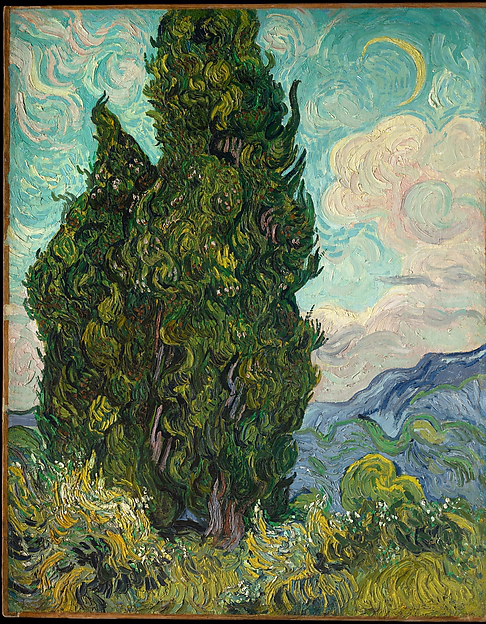
\includegraphics[scale=0.4]{images/cypres.png}
\end{center}
\end{minipage}\hfill
\begin{minipage}{0.3\linewidth}
\begin{center}
\textbf{Image cachée}

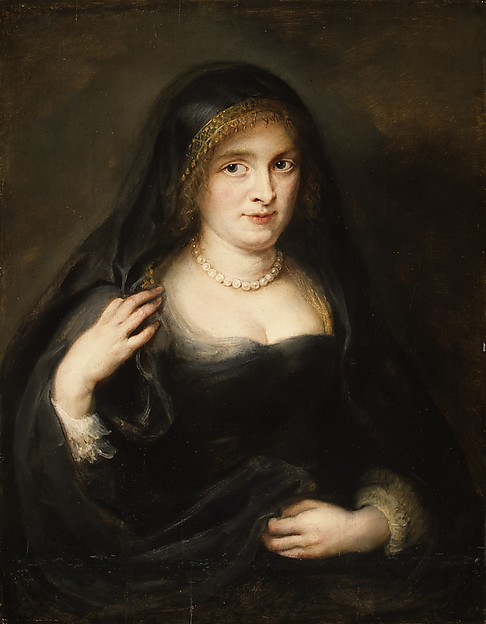
\includegraphics[scale=0.4]{images/femme.png}
\end{center}
\end{minipage}\hfill
\hfill
\begin{minipage}{0.3\linewidth}
\begin{center}
\textbf{Image dévoilée}

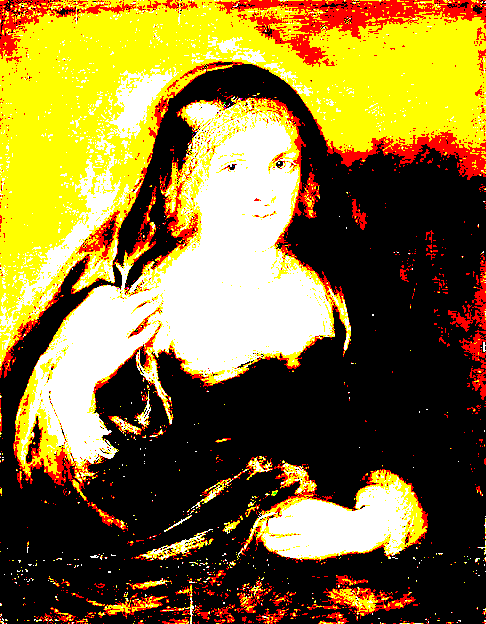
\includegraphics[scale=0.4]{images/femme-devoile.png}
\end{center}
\end{minipage}

Pour réaliser cette opération, nous allons utiliser les représentations binaires des valeurs des pixels, et en particulier des opérateurs bit à bit, que nous présentons brièvement ci-dessous :   



\begin{methode}{Opérateurs bit à bit}
Pour convertir un entier en une série de bits, il suffit de l'écrire en base $2$, on parle d'\textit{écriture binaire}. 

L'\textit{écriture décimale }de treize est $13$ car $1 \times 10 + 3 = 13$.

Son  \textit{écriture binaire}  est $(1101)_{2}$ car $1 \times 2^{3} + 1 \times 2^{2} + 0 \times 2^{1} + 1 \times 2^{0} = 13$.

\begin{itemize}
\item En Python la fonction \texttt{bin} retour l'écriture binaire d'un entier sous forme de chaîne de caractère préfixée de '0b' et sa réciproque est la fonction \texttt{int} avec le paramètre optionnel $2$.
\begin{lstlisting}[numbers=none]

In [92]: bin(13)
Out[92]: '0b1101'

In [93]: int('0b1101', 2)
Out[93]: 13
\end{lstlisting}

\item L'opérateur \texttt{>>} permet de décaler les bits vers la droite, tandis que \texttt{<<} les décale vers la gauche :
\begin{lstlisting}[numbers=none]
In [94]: 13 >> 1
Out[94]: 6

In [95]: bin(6)
Out[95]: '0b110'

In [96]: 13 << 1
Out[96]: 26

In [97]: bin(26)
Out[97]: '0b11010'
\end{lstlisting}

\item L'opérateur \verb+&+ permet de réaliser une opération logique ET bit par bit entre deux entiers, tandis que l'opérateur \verb+|+ permet de réaliser une opération logique OU bit par bit  entre deux entiers:

\medskip

\begin{minipage}{0.4\linewidth}
\begin{center}
\textbf{Table de vérité du ET}

\medskip
\begin{tabular}{|c|c|c|}
\hline
x &  y & x ET y \\
\hline
0 & 0 &  0 \\
\hline
0 & 1 & 0 \\
\hline
1 & 0 & 0 \\
\hline
1 & 1 & 1\\
\hline
\end{tabular}
\end{center}
\end{minipage}\hfill
\begin{minipage}{0.4\linewidth}
\begin{center}
\textbf{Table de vérité du OU}

\medskip
\begin{tabular}{|c|c|c|}
\hline
x &  y & x OU y \\
\hline
0 & 0 & 0  \\
\hline
0 & 1 &  1 \\
\hline
1 & 0 & 1 \\
\hline
1 & 1 & 1 \\
\hline
\end{tabular}
\end{center}
\end{minipage}

\bigskip

\begin{lstlisting}
In [101]: bin(13), bin(10)
Out[101]: ('0b1101', '0b1010')

In [102]: 13 & 10, bin(13 & 10)
Out[102]: (8, '0b1000')

In [103]: 13 | 10, bin(13 | 10)
Out[103]: (15, '0b1111')
\end{lstlisting}
\end{itemize}

On utilise souvent le ET binaire avec un entier particulier appelé \textit{masque} qu'on applique à un autre entier pour faire apparaître  une information par \og{} gommage  \fg{} des bits  qui ne sont pas égaux à $1$ comme dans le \textit{masque}. Ce peut être pour récupérer l'adresse IP du sous-réseau dont dépend une machine (voir \url{https://fr.wikipedia.org/wiki/Sous-réseau} ) ou pour fixer des droits par défaut à tout  fichier créé en appliquant le masque à la série  $111111111$ représentant les droits RWXRWXRWX en lecture (R), écriture (W), exécution (X) pour le propriétaire, le groupe principal ou les autres utilisateurs du fichier.
\end{methode}

\begin{methode}{Application à la stéganographie}
On va créer une image C contenant à la fois les images A et B, et l'apparence de C sera celle de A car les informations extraites de A seront placées au \og{} premier plan \fg{} dans le codage numérique de chaque pixel  :

\begin{itemize}[label=\ding{43}]

\item Soit $a$ la valeur d'une des trois composantes (R,G,B) d'un pixel de l'image A et  $b$  et $c$ les valeur de la même composante du même pixel respectivement dans  les images B et C.

$a$ et $b$ sont des entiers compris entre  entre $0$ et $255$ dont la représentation binaire compte $8$ bits.

Lorsqu'on lit de gauche à droite une écriture binaire de 8 bits, les  premiers bits lus sont dits de \textit{poids forts} et les derniers de \textit{poids faibles}. 

\item Pour construire les $8$ bits de $c$, on prend par exemple les $5$ bits de poids forts de $a$ suivis des $8-5=3$ bits de poids forts de $b$. On perd de l'information sur $a$ et $b$ : plus on prend  de bits de poids forts moins la perte est importante pour $b$ mais plus l'apparence de l'image C s'éloigne de celle de A.

Par exemple avec $a=166$ d'écriture binaire $a = (\overbrace{10100}^{\text{forts}}110)_{2}$  et $b=234$ d'écriture binaire $b=(\underbrace{111}_{{\text{forts}}}01010)_{2}$, on construit $c= (\overbrace{10100}^{a}\underbrace{111}_{b})_{2}$

\begin{itemize}
 \item Pour annuler les $3$ bits de poids faible de $166$ on fait  d'abord un ET logique entre $166$ et le nombre \og{} masque \fg{} d'écriture binaire $(11111000)_{2}$ qui est  $248$, on obtient $(10100000)_{2}$. 

\item Ensuite on décale de $5$ bits vers la droite les bits de l'écriture binaire de $234$ avec $234>>5$ ce qui permet de les obtenir comme bits de poids faibles du nombre d'écriture binaire $(111)_{2}$ (c'est 7). 

\item Enfin on effectue un OU logique entre $(\overbrace{10100}\underbrace{000})_{2}$ et $(\underbrace{111})_{2}$ et on obtient la réunion de tous ces bits : $c=(\overbrace{10100}\underbrace{111})_{2}$ avec les trois bits de poids forts de $b=234$ à la place des trois bits de poids faibles de $a=166$.

\item On peut réaliser les mêmes opérations  avec les opérateurs de division euclidienne \verb+//+ et \verb+%+ :

\begin{lstlisting}[style=compil]
In [11]: a, b, nbits = 166, 234, 5                                              

In [12]: masque = (255 >> (8 - 5)) << (8 - 5)                                   

In [13]: bin(a), bin(b), bin(masque)                                            
Out[13]: ('0b10100110', '0b11101010', '0b11111000')

In [14]: c = (a & masque) | (b >> 5)                                             

In [15]: bin(c)                                                                 
Out[15]: '0b10100111'

In [16]: c, bin(c)                                                              
Out[16]: (167, '0b10100111')

In [17]: (a & masque) == (a // 2**(8-5)) * 2 ** (8 - 5)                         
Out[17]: True

In [18]: (b >> 5) == (b // 2 ** 5)                                              
Out[18]: True

In [19]: c == (a // 2**(8-5)) * 2 ** (8 - 5) + (b >> 5)                         
Out[19]: True

In [20]: (c << 5) & 255 == (c % 2 ** (8 - 5)) * 2 ** 5                          
Out[20]: True
\end{lstlisting}

\end{itemize}

\end{itemize}


\end{methode}

\begin{enumerate}
	\item Écrire les fonctions dont on donne les prototypes ci-dessous :
	
\begin{lstlisting}[style=rond]
def cacher_image(pix_visible, pix_invisible, mode):
    """Prend en paramètres :
    - 2 matrices de pixels pix_visible et  pix_invisible de mêmes dimensions et profondeur
    - mode de type str pour désigner la  profondeur de l'image  ('L' ou 'RGB')
    Retourne une matrice de pixels pix_but de mêmes dimensions et profondeur que pix_visible
    l'ecriture binaire d'une composante de pix_but[y][x] est constituée ainsi !
    5 bits de poids forts =  5 bits de poids fort de la composante de pix_visible[y][x]
    3 bits de poids faible =  3 bits de poids fort de la composante de pix_invisible[y][x]
    """
    
def extraire_image(pix, mode):
    """Prend en paramètres :
    - pix qui est 1 matrice de pixels 
    - mode de type str pour désigner la  profondeur de l'image  ('L' ou 'RGB')
    Retourne une matrice de pixels pix_but de mêmes dimensions et profondeur que pix
    Les 3 bits de poids forts d'une composante de pix_but[y][x] 
    sont les 3 bits de poids faible de pix[y][x]
    """
\end{lstlisting}

\item Écrire deux fonctions similaires qui prennent chacune un paramètre supplémentaire \texttt{nbits} qui correspond au nombre de bits de poids forts conservés dans l'image visible (5 dans la version précédente).

\item Écrire deux fonctions de même signatures que les précédentes mais qui utilisent les opérateurs de division euclidienne plutôt que les opérateurs bit à bit.

\item Proposer une interface graphique avec Tkinter.

Voir \url{https://www.geeksforgeeks.org/loading-images-in-tkinter-using-pil/} pour une intégration d'images PIL dans Tkinter.
\end{enumerate}



\subsubsection{Sujet 2 : traitement d'image, filtres de Sobel (\textit{moyen})}


On ne travaille que sur des images en nuances de gris.

\begin{minipage}{0.45\linewidth}

\begin{center}
\fbox{Matrice de convolution}
\begin{tikzpicture}[thick, scale=2.5]
\draw (-1,-1) grid (2,2);
\foreach \u/\v/\w in {-0.5/1.5/a,-0.5/-0.5/g,-0.5/0.5/d, 0.5/-0.5/h, 0.5/1.5/b, 1.5/0.5/f,1.5/1.5/c,1.5/-0.5/i}
\draw (\u, \v) node {$\w$};
\draw (0.5, 0.5) node {$e$};
\draw[->, >=latex] (-1,2) -- (2.1,2);
\draw[->, >=latex] (-1,2) -- (-1,-1.1);
\end{tikzpicture}
\end{center}

\end{minipage}\hfill
\begin{minipage}{0.45\linewidth}

\begin{center}
\fbox{Voisinage du pixel de coordonnées $(x,y)$}
\begin{tikzpicture}[thick, scale=2.5]
\draw (-1,-1) grid (2,2);
\foreach \u/\v/\dx/\dy in {-0.5/1.5/-1/-1,-0.5/-0.5/-1/+1,-0.5/0.5/-1/+0, 0.5/-0.5/+0/+1, 0.5/1.5/+0/-1, 1.5/0.5/+1/+0,1.5/1.5/+1/-1,1.5/-0.5/+1/+1}
\draw (\u, \v) node {$(x  \dx, y  \dy)$};
\draw (0.5, 0.5) node {$(x,y)$};
\draw[->, >=latex] (-1,2) -- (2.1,2);
\draw[->, >=latex] (-1,2) -- (-1,-1.1);
\end{tikzpicture}
\end{center}
\end{minipage}

Le \href{https://fr.wikipedia.org/wiki/Filtre_de_Sobel}{filtre de Sobel} est un filtre de détection de contour qui fait appel à des opérations de convolution entre le voisinage carré $3 \times 3$ d'un pixel de coordonnées $(x,y)$ et deux matrices de coefficients  de mêmes dimensions.

On calcule ainsi une approximation du gradient de l'intensité du pixel, équivalent de la dérivée dans un espace à deux dimensions. Ce gradient mesure donc la variation d'intensité au voisinage du pixel et il est d'autant plus  grand et proche de 255 (blanc) si le pixel est sur un contour.  


Avec les notations du schéma ci-dessus le produit de convolution de la matrice de coefficients à gauche par le voisinage du pixel à droite s'obtient comme une somme des  produits de coefficients par les pixels en même position. On note $\text{pix}[y][x]$ le pixel d'abscisse $x$ et d'ordonnée $y$.

\begin{multline*}
a \times \text{pix}[y-1][x-1] + b \times \text{pix}[y-1][x] + c \times \text{pix}[y-1][x+1] \\
+ d \times \text{pix}[y][x-1] + e \times \text{pix}[y][x] + f \times \text{pix}[y][x+1]  \\
+ g \times \text{pix}[y+1][x-1] + h \times \text{pix}[y+1][x] + i \times \text{pix}[y+1][x+1] 
\end{multline*}


Par exemple le produit de convolution de la matrice de coefficients $A=\begin{pmatrix} 1 & 2 & 1 \\ 2 & 4 & 2 \\ 1 & 2 & 1 \end{pmatrix}$ par le voisinage de pixels $B=\begin{pmatrix} 50 & 10 & 80 \\ 60 & 40 & 20 \\ 70 & 30 & 90 \end{pmatrix}$ est $1 \times 50 + 2 \times 10 + 1 \times 80 + 2 \times 60 + 4 \times 40 + 2 \times 20 + 1 \times 70 + 2 \times 30 + 1 \times 90$.


Le \href{https://fr.wikipedia.org/wiki/Filtre_de_Sobel}{filtre de Sobel} calcule d'abord pour chaque pixel de coordonnées $(x,y)$ les produits de convolution de son voisinage carré $3 \times 3$ par les matrices $C=\begin{pmatrix} -1 & 0 & 1 \\ -2 & 0 & 2 \\ -1 & 0 & 1 \end{pmatrix}$ pour la variation d'intensité horizontale et  $D=\begin{pmatrix}  -1 & -2 & -1 \\ 0 & 0 & 0 \\ 1 & 2 & 1 \end{pmatrix}$ pour la variation d'intensité verticale. En notant $p_{h}$ et $p_{v}$ ces deux produits,  on calcule ensuite leur norme euclidienne $\sqrt{p_{h}^{2}+p_{v}^{2}}$. Enfin  on la normalise pour avoir une valeur entière entière entre 0 et 255, en prenant sa partie  entière et  en minorant par 255 si elle excède 255.

Voici un exemple :

\begin{minipage}{0.45\linewidth}
\begin{center}
\textbf{Original}
 
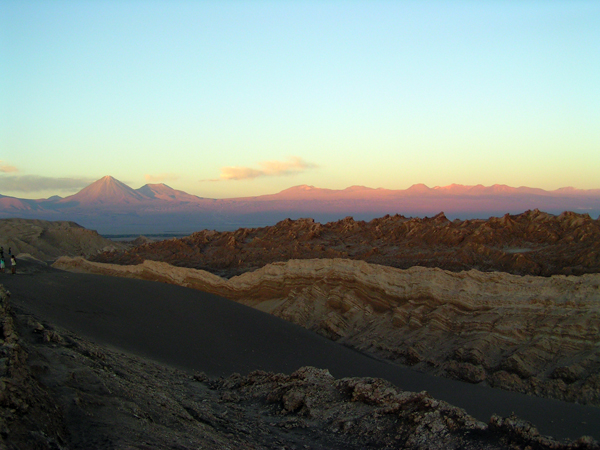
\includegraphics[scale=0.3]{images/valleluna.jpg}
\end{center}
\end{minipage}\hfill
\begin{minipage}{0.45\linewidth}
\begin{center}
\textbf{Contour Sobel}

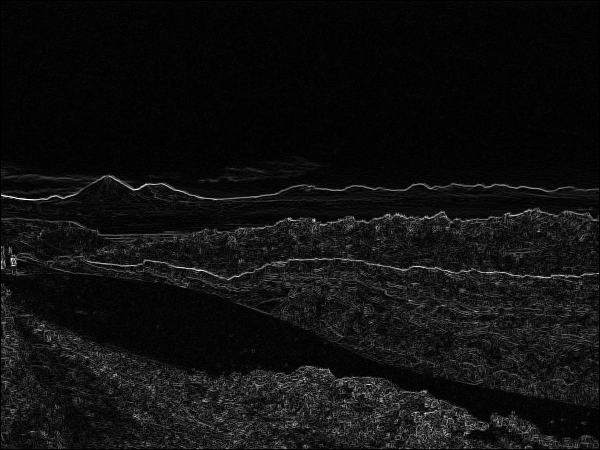
\includegraphics[scale=0.3]{images/valleluna-contour-sobel.png}
\end{center}
\end{minipage}

\begin{enumerate}
	\item Écrire les fonctions dont on donne les prototypes ci-dessous :
\begin{lstlisting}[style=rond]
from math import sqrt

def moyenne_rgb(pixel, coef):
	"""Prend en paramètres :
	- pixel un tableau de trois entiers entre 0 et 255 représentant un pixel RGB
	- coef un tableau de 3 nombres positifs
	Retourne un entier qui est la partie entière
	de la moyenne pondérée des composantes RGB de pixel par les coefficients de coef
	"""
    

def monochrome(pix, coef):
    """Prend en paramètres :
    - pix une matrice de pixels RGB
    - coef un tableau de 3 nombres positifs
    Retourne une matrice de pixels pix_but représentant la conversion
    en nuances de gris de l'image de  pix,
    avec les coefficients de pondération coef"""
    

def detection_contour(pix, filtre_contour):
    """Prend en paramètres :
    - pix une matrice de pixels RGB
    - filtre_contour une fonction qui peut modifier la valeur d'un pixel 
      en marquant les pixels de contour, les pixels du bord ne sont pas traités
    Retourne une nouvelle matrice de pixels pix_but
    obtenue en appliquant filtre_contour à chaque pixel de coordonnées (x,y)""" 
    
sobel_vertical = [[-1, -2, -1],
                   [0,0,0],
                   [1, 2, 1]]

sobel_horizontal = [[-1,0,1],
                    [-2,0,2],
                    [-1,0,1]]
                    
def normalise(val):
    """Prend en paramètre un nombre val
    Retourne 0 si val <= 0
    partie entière de val si 0 <= val <= 255 
    et 255 sinon"""
    

def convolution_bloc3(pix, x,y, mat_conv): 
	"""Prend en paramètres :
	- pix une matrice de pixels
	- x et y deux entier désignant les coordonnées d'un pixel de pix
	- mat_conv une matrice de convolution 3 x 3
	Retourne le produit de convolution de mat_conv
	par le voisinage carré 3x3 du pixel en (x,y)
	Contrainte : utiliser un seul opérateur +
	"""
    

def filtre_contour_sobel(pix, x, y):  
    """Prend en paramètres :
	- pix une matrice de pixels
	- x et y deux entier désignant les coordonnées d'un pixel de pix
	Retourne l'entier  calculé par le filtre de Sobel
    pour le pixel en (x, y), voir l'énoncé
    et https://fr.wikipedia.org/wiki/Filtre_de_Sobel"""
\end{lstlisting}
\end{enumerate}

\subsubsection{Sujet 3 : programmation d'un jeu de pendu (\textit{facile})}


\begin{itemize}[label=\ding{223}]

	\item L'ordinateur choisit aléatoirement un mot dans le fichier \texttt{dicoSansAccents.txt} fourni.
	
	\item Le joueur  doit deviner le mot en un nombre fixé de tours, à chaque tour il peut choisir entre la  proposition d'une lettre ou du mot complet. Si le lettre proposée  se trouve dans le mot l'ordinateur affiche le mot avec les lettres trouvées ou des tirets bas à la place des lettres non découvertes. Si le lettre a déjà été proposée ou si elle n'appartient pas au mot, l'ordinateur le signale au joueur. La boucle se termine si le joueur a proposé le mot ou si le nombre de tours maximal  est atteint.
	
	\item A la fin de la partie, l'ordinateur affiche un message de conclusion.	
 
	\item Proposer une petite interface graphique avec Tkinter.
\end{itemize}
	
	
	 
\subsubsection{Sujet 4 : programmation d'un moteur basique de système de saisie prédictive T9 utilisé sur les téléphones mobiles à touches (\textit{moyen})}


\begin{center}
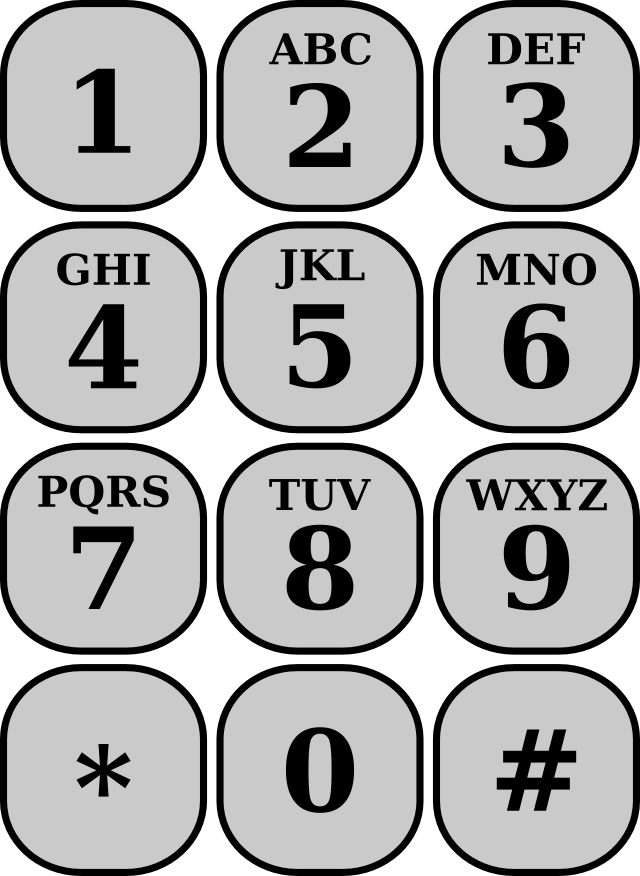
\includegraphics[scale=0.15]{images/Telephone-keypad.png}

\uline{Source} : CC BY-SA 3.0, \url{https://commons.wikimedia.org/w/index.php?curid=111558}
\end{center}

Voici le cahier des charges :

\begin{enumerate}



	\item Lire l'article de Wikipedia sur ce système \url{https://fr.wikipedia.org/wiki/Saisie_intuitive#T9}.
	
	\item Récupérer auprès de l'enseignant le fichier \texttt{motsFrSansAccents.txt} qui contient la liste des fréquences par million d'occurrences de \np{123150} mots sans accents de la langue française. Ce fichier a été constitué à partir du fichier \verb+liste_mots.txt+ récupéré sur le site \url{http://www.lexique.org}.
	

\begin{lstlisting}
def fichier2dico(fichier, delimiteur = '\t', charset = 'latin1'):  
	"""Parcourt  un fichier comme motsFrSansAccents.txt 
	Renvoie un dictionnaire Python associant à chaque mot sa fréquence."""  
\end{lstlisting}
 
	
\begin{lstlisting}
In [9]: dico = fichier2dico('motsFrSansAccents.txt')

In [10]: dico['la']
Out[10]: 25094.9
\end{lstlisting}

  \item Écrire une fonction \texttt{mot2code} qui prend en argument un mot sans accent et qui renvoie son codage T9 sous la forme d'une chaîne de caractères.
  
\begin{lstlisting}
In [33]: mot2code('python')
Out[33]: '798466'
\end{lstlisting}
  
 \item Écrire une fonction \texttt{listPrefixe(mot)} qui prend en argument un mot et qui renvoie la liste de tous ses préfixes.
 
\begin{lstlisting}
In [34]: listPrefixe('python')
Out[34]: ['p', 'py', 'pyt', 'pyth', 'pytho', 'python']
\end{lstlisting}
 
 \item Écrire une fonction \texttt{dico2freq(dico)}. 
 
 Elle prend en argument un dictionnaire Python, des fréquences de mots, retourné par la fonction \\
 \texttt{fichier2dico}, et elle renvoie un dictionnaire qui associe à une chaîne de caractères, la somme des fréquences des mots qu'elle préfixe. On parle de poids du préfixe.
 
\begin{lstlisting}
In [35]: freq = dico2freq(dico)

In [36]: freq['scie']
Out[36]: 254.38000000000002
\end{lstlisting}

\item Écrire une fonction \texttt{freq2proposition(freq)}, qui prend en argument un dictionnaire \texttt{freq} retourné par la fonction \texttt{dico2freq} et qui retourne un dictionnaire associant à chaque séquence de touche saisie sur un clavier T9 la chaîne de caractères qu'elle code et qui constitue un préfixe de poids maximal.

Par exemple, la séquence de touches \texttt{'7243'} peut coder \texttt{'scie'} ou \texttt{'chaîne'} mais \texttt{'scie'} est le préfixe de poids maximal pour cette séquence \footnote{D'après notre fichier \texttt{motsFrSansAccents.txt}}, c'est donc la proposition choisie. En pratique, le logiciel du téléphone permet de parcourir la liste des préfixes dans l'ordre décroissant de leur poids.
\begin{lstlisting}
In [37]: prop = freq2proposition(freq)

In [38]: prop['7243']
Out[38]: 'scie'

In [39]: freq['scie']
Out[39]: 254.38000000000002

In [40]: freq['sage']
Out[40]: 57.41 
\end{lstlisting}


\item Proposer une interface graphique avec Tkinter : clavier T9 et affichage du mot le plus probable.

\end{enumerate}



\subsubsection{Sujet 5 : chiffrements de César et Vigenère  (\textit{moyen})}


\begin{itemize}

\item La \textbf{cryptographie} (du grec \textit{kruptos} : caché, et \textbf{graphein} : écrire) qui est l'art de coder le message d'une façon connue uniquement de l'émetteur et du récepteur. On appelle  \textbf{chiffre} un procédé de cryptage d'un texte caractère par caractère.

\item D'après la légende,  César aurait chiffré sa correspondance avec un  \textbf{chiffre par substitution monoalphabétique} : chaque lettre de l'alphabet est remplacée dans le texte chiffré par une autre lettre, toujours la m\^eme. Il existe aussi des  \textbf{chiffres par substitution polyalphabétique} comme le chiffre de Vigenère : chaque lettre de l'alphabet est remplacée dans le texte chiffré par une autre lettre, mais qui varie selon la position dans le message.

 Dans le  chiffre de César, chaque lettre du texte chiffré s'obtient par un décalage de la lettre du texte en clair. Ce décalage est la clef du chiffre, pour le chiffre de César cette clef est 3 : A est chiffré par D, B par E,W par Z et X par A.

Notre alphabet comptant 26 lettres, on peut repérer  A par 0, B par 1 \ldots Z par 25. 

Le chiffre de César peut alors se modéliser sous la forme d'une fonction mathématique qui à une lettre en clair repérée par $x$ avec $0\leqslant x \leqslant 25$ associe une lettre chiffrée repérée par $y \equiv x+3 \text{ mod } 26$.

Cette notation se lit $y$ congru à $x+3$ modulo 26 et signifie que  $y$ est égal au  reste de la division euclidienne de $x+3$ par 26. On peut changer la clef de décalage et si on prend $13$ on obtient le chiffrement \texttt{rot13} déjà rencontré.

\begin{center}
\begin{tabular}{|c|c|c|c|c|c|c|c|}
\hline 
Lettre en clair & A & B & \ldots & W & X & Y & Z \\ 
\hline 
$x$ & 0 & 1 & \ldots & 22 & 23 & 24 & 25 \\ 
\hline 
$y \equiv x+3 \text{ mod } 26$& 3 & 4 & \ldots & 25 & 0 & 1 & 2 \\ 
\hline 
Lettre chiffrée & D & E & \ldots & Z & A & B & C \\ 
\hline 
\end{tabular} 
\end{center}

\item Pour déchiffrer un message codé par le chiffre de César, si le message comporte suffisamment de caractères, on peut procéder par \textit{analyse fréquentielle}. 

On recherche la clef de déchiffrement, entre $0$ et $25$, qui minimise la distance entre l'histogramme du texte déchiffré et l'histogramme de répartition des lettres dans la langue ciblée.

Par exemple, en Français, la liste des fréquences des lettres minuscules de \texttt{'a'} d'indice $0$ à \texttt{'z'} d'indice $25$ est :

\begin{lstlisting}
freqref = [8.4, 1.06, 3.03, 4.18, 17.26, 1.12, 1.27, 0.92, 7.34, 0.31, 0.05, 6.01, 2.96, 7.13, 5.26, 3.01,0.99, 6.55, 8.08, 7.07, 5.74, 1.32, 0.04, 0.45, 0.3, 0.12]
\end{lstlisting}


\item Le chiffre de Vigenère est un \textbf{chiffre de substitution polyalphabétique} : chaque lettre en clair est remplacée par une lettre chiffrée mais cette traduction varie selon la position de la lettre en clair dans le message.


Il s'agit d'un chiffre de César dont le décalage change selon la position de la lettre en clair dans le message.

Par exemple, soit le texte en clair  IL FAIT BEAU et la clef PLUIE. 

Sur la première ligne on  écrit le texte en clair sans espaces, sur la deuxième  on répète la clef sur la m\^eme longeur, sur la troisième on écrit le texte chiffré:

\begin{center}
ILFAITBEAU

PLUIEPLUIE

XWZIMIMYIY
\end{center}

Pour chaque lettre en clair, le rang de la lettre de la clef en dessous donne le décalage qu'on  applique pour déterminer la lettre chiffrée. Les rangs varient de 0 pour A à 25 pour Z.

\begin{description}
\item P de rang 15 en dessous de I donc I décalée de 15 donne  X
\item L de rang 11 en dessous de L donc L décalée de 11 donne   W
\item U de rang 20 en desous de F donc F décalée de 20 donne Z \dots
\end{description}

\end{itemize}


Voici le cahier des charges :

\begin{itemize}[label=\ding{223}]

	\item Compléter le code de la fonction \texttt{chiffreCesar(source, decalage)} ci-dessous qui prend en argument une chaîne de caractères \texttt{source} et  \texttt{decalage}  un entier entre $0$ et $25$. La chaîne \texttt{source} ne doit pas comporter de caractères diacritiques, elle est convertie d'abord  en majuscules, puis une chaîne  \texttt{sortie} est construite en remplaçant chaque caractère alphabétique par son image par le chiffre de César de clef \texttt{decalage}. 
	
\begin{lstlisting}
def chiffreCesar(source, decalage):
	source = source.upper()
    sortie = ''
    for c in source:
        if c.isalpha():
            #à compléter
        else:
            sortie += c
    return sortie
\end{lstlisting}

\item Écrire une fonction \texttt{dechiffreCesarClef(source, decalage)} où \texttt{decalage} est la clef de chiffrement utilisée.

\begin{lstlisting}
In [10]: chiffreCesar('Un python est un serpent constricteur.', 1)
Out[10]: 'BU WFAOVU LZA BU ZLYWLUA JVUZAYPJALBY.'

In [11]: dechiffreCesarClef('BU WFAOVU LZA BU ZLYWLUA JVUZAYPJALBY.', 1)
Out[11]: 'GZ BKFTAZ QEF GZ EQDBQZF OAZEFDUOFQGD.'
\end{lstlisting}

\item Écrire une fonction \texttt{calculerFrequence(source)} qui retourne l'histogramme des fréquences (en \%) des $26$ caractères alphabétiques,  dans une chaîne de caractères \texttt{source} composée de caractères non accentués et en majuscules.

\item Écrire une fonction \texttt{calculerDistance(freq1, freq2)} qui calcule la distance euclidienne entre deux listes d'histogrammes de fréquences des  $26$ caractères alphabétiques.

Si on note $\left( f_{i} \right)_{0 \leqslant i \leqslant 25}$ et $\left( g_{i} \right)_{0 \leqslant i \leqslant 25}$ les séries de fréquences des deux histogrammes, la distance euclidienne entre les deux histogrammes est égale à :
\begin{equation*}
\sqrt{\left(f_{0} - g_{0}  \right)^{2} + \left(f_{1} - g_{1}  \right)^{2} + \cdots + \left(f_{25} - g_{25}  \right)^{2}}
\end{equation*}


\item Écrire une fonction \texttt{calculerDecalage(source, freqref)}, qui prend en argument une chaîne de caractères \texttt{source}  et une liste \texttt{freqref} représentant l'histogramme des caractères alphabétiques  dans la langue ciblée (voir ci-dessus pour le Français). Cette fonction doit retourner le décalage entre $0$ et $26$ pour lequel l'histogramme de l'image de \texttt{source} par le chiffre de César présente une distance minimale avec \texttt{freqref}.

En déduire une fonction \texttt{dechiffreCesar(source, freqref)} qui déchiffre un message crypté par le chiffre de César.


Tester ces fonctions avec le contenu du fichier texte \texttt{clair.txt} qui contient le début du roman \og{} \textit{Les trois mousquetaires} \fg{}.

\begin{lstlisting}
In [34]: f = open('clair.txt','r')

In [35]: message = f.read().upper()

In [36]: chiffre = chiffreCesar(message, 3)

In [38]: dechiffreCesar(chiffre, freqref) == message
Out[38]: True
\end{lstlisting}

\item Écrire une fonction \texttt{chiffreVigenere(source, clef)} qui chiffre  une chaîne de caractère \texttt{source} avec le chiffre de Vigenère pour une \texttt{clef} donnée.

En déduire une fonction \texttt{chiffreVigenereClef(source, clef)} qui déchiffre une chaîne de caractères cryptée avec le chiffre de Vigenère pour une \texttt{clef} donnée.

\begin{lstlisting}
In [62]: chiffreVigenere('AMSTERDAM', 'ROME')
Out[62]: 'RAEXVFPED'

In [63]: dechiffreVigenereClef('RAEXVFPED', 'ROME')
Out[63]: 'AMSTERDAM'
\end{lstlisting}


\item Proposer une petite interface graphique en Tkinter qui permette de chiffre ou déchiffre un texte saisi par l'utilisateur  avec le chiffre de César ou celui de Vigenère.

\end{itemize}


\subsection{8 Sujets non guidés}


\begin{itemize}

\item \textbf{Chou, Chèvre, Loup} $\Rightarrow$ \textit{Moyen}


\medskip


À partir de la ressource \url{https://alainbusser.frama.io/NSI-IREMI-974/WGC.html}, résoudre le problème \textbf{Chou, Chèvre, Loup}  sans utiliser le paradigme de programmation objet ni l'instruction \texttt{exec}.

Proposer une interface graphique en Tkinter permettant à un joueur de choisir un déplacement du  chou, de la chèvre ou du  loup d'une rive à l'autre, lui indiquant si ce déplacement est possible et le félicitant s'il résout le problème.


\bigskip

\item \textbf{Le jeu de la vie} $\Rightarrow$ \textit{Moyen}

\medskip

Sur un damier carré, on dispose des créatures de manière aléatoire. La population évolue d'un état au suivant selon les règles suivantes :
\begin{itemize}
\item une créature survit si elle a 2 ou 3 voisines dans les 8 cases adjacentes et elle meurt à cause de son isolement ou de la surpopulation sinon,
\item une créature naît dans une case vide s'il y a exactement 3 créatures dans les 8 cases voisines, et rien ne se passe dans cette case sinon.
\end{itemize}
Écrire avec la bibliothèque Tkinter de Python un  programme qui simule le développement d'une population.

Voir \url{https://www.academie-sciences.fr/fr/Seances-publiques/le-jeu-de-la-vie.html}.

\bigskip

\item \textbf{Jeu de Pong}   $\Rightarrow$ \textit{Difficile}

\medskip

Écrire une version Python du jeu Pong (ou de Space Invaders, Snake \ldots) On utilisera la bibliothèque Tkinter pour Python.

\bigskip



\item \textbf{Jeu de puissance 4} $\Rightarrow$ \textit{Difficile}

\medskip

Réaliser une version du jeu de Puissance 4 pour 2 joueurs avec interface graphique.


Prolongement possible : un joueur joue contre l'ordinateur.  


\bigskip 


\item \textbf{Princesse de Clèves en Emoji}  $\Rightarrow$ \textit{Moyen}

Niveau 1 du sujet proposé par Laurent Abbal sur \url{https://github.com/hackathon-nsi/h7n-nsi-02}.

\begin{itemize}
\item     Lire l'article Wikipedia sur les Émoji.
 \item   Revoir les encodages ASCII et Unicode.
  \item   Visiter et étudier : \url{https://unicode.org/emoji/charts/full-emoji-list.html}
   \item  Étudier la première partie de La Princesse de Clèves et faire une première liste de termes qui pourraient être remplacés par des Émoji.
   \item Implémenter deux algorithmes de recherche d'un motif dans un texte :
   	\begin{itemize}
   		\item l'algorithme naif
   		\item l'algorithme de Boyer-Moore Horspool.  
\end{itemize}   	 
Voir \href{https://cache.media.eduscol.education.fr/file/NSI/63/5/RA20_NSI_G_T_boyer-moore_1298635.pdf}{ce document}

et \url{https://pixees.fr/informatiquelycee/n_site/nsi_term_algo_boyer.html}.
   \item  Écrire un programme en Python qui remplace les termes de la liste précédente par les Émojis correspondants en utilisant l'algorithme de Boyer-Moore Horspool.
  \end{itemize}



\bigskip

\item \textbf{Fractales et L-systèmes} $\Rightarrow$ \textit{Facile}

Écrire un programme avec un interface graphique qui permet de saisir un motif initial puis des règles de réécriture et quelques paramètres graphiques puis  trace des représentations approchées de fractales selon un algorithme de \href{https://fr.wikipedia.org/wiki/L-Syst\%C3\%A8me}{L-système} : flocon de Von Koch, triangle de Sierpinski \ldots 

Proposer une petite interface graphique avec Tkinter.

\bigskip

\item \textbf{Réalisation d'une calculatrice en notation Polonaise inverse} $\Rightarrow$ \textit{Difficile}

\medskip

\begin{itemize}

 \item Écrire un programme d'émulation de calculatrice qui effectue des calculs  élémentaires (addition, soustraction, multiplication, division) en notation \textit{postfixée} ou \textit{ polonaise inverse}. Proposer une petite interface graphique en Tkinter. Commencer par résoudre ce problème : \url{https://www.codingame.com/ide/puzzle/reverse-polish-notation}
 
 \item Rajouter une fonctionnalité qui traduit une expression en notation postfixée dans une  expression en notation infixée avec  un nombre minimal de parenthèses. Commencer par résoudre ce problème : \url{https://www.codingame.com/training/medium/the-polish-dictionary}.
 
 \end{itemize}

 \bigskip
 
 
\item \textbf{Sudoku} $\Rightarrow$ \textit{Difficile}
 
\medskip

Réaliser un solveur de Sudoku  par backtracking, avec ou sans interface graphique.  Source : le problème 1 de \url{https://www.apmep.fr/IMG/pdf/CAPES_avril_2017_epreuve_info.pdf}. 



\end{itemize}

\section{Quelques bibliothèques de Python qui pourraient vous \^etre utiles}

\begin{itemize}[label=\ding{43}]



\item Réalisation d'interfaces graphiques plut\^ot statiques : \textbf{tkinter} (sous Python 3) ou \textbf{Tkinter} (Python2) :

\url{http://infohost.nmt.edu/tcc/help/pubs/tkinter/web/index.html}
\item Traitement d'images : \textbf{PIL} ou son fork \textbf{Pillow} : \url{https://pypi.python.org/pypi/Pillow/}

 \item Bibliothèques pour le calcul scientifique : \textbf{numpy} ou plus généralement \textbf{scipy} : 
 
 \url{http://scipy.org/}
 
 \item Réalisation de graphiques pour les mathématiques ou la physique (possibilité d'animation) : \textbf{matplotlib} :
  \url{http://matplotlib.org/}
 
\item Collecte de données sur le Web :

\begin{itemize}
\item  récupérer les données avec \textbf{requests} : \url{https://realpython.com/python-requests/} 
\item    \og{} parser \fg{} du HTML  avec \textbf{beautiful soup} : 
\url{https://realpython.com/beautiful-soup-web-scraper-python/}.
\end{itemize}

\end{itemize}


\section{Quelques outils pour la gestion de projet ou le travail collaboratif}

\begin{itemize}[label=\ding{43}]

\item Cours et ressources en ligne sur \url{https://parc-nsi.github.io/premiere-nsi/}.

\item Vous pouvez créer un dépôt privé de fichiers sur \href{https://github.com}{Github} ou \href{https://gitlab.com/}{Gitlab}. Pour l'utilisation de git, voir cette \url{https://rogerdudler.github.io/git-guide/index.fr.html}.


\item Partage de fichiers, pad, articles de  blog, notebooks Python  dans  l'ENT : \url{https://le-parc.ent.auvergnerhonealpes.fr/}

\item Partage de scripts Python et test en ligne : \url{https://console.basthon.fr/}.

\item Documents textuels collaboratifs (avec possibilité de chat) : \textbf{Framapad} accessible depuis  \url{https://framapad.org/}.

\item Feuilles de calculs collaboratives  : \textbf{Framacalc} accessible depuis  \url{https://framacalc.org/}.


\item Réalisation de carte mentale   : \textbf{Framindmap} accessible depuis \url{https://framindmap.org/c/maps/}.


\end{itemize}

\newpage

\begin{center}

{\large \textbf{ANNEXE 1 : Fiche de suivi du projet  (à remplir pour le premier point étape)}}

\vspace{0.5 cm}
{\small

\begin{tabular}{|p{0.2\linewidth}|>{\centering \arraybackslash}p{0.5\linewidth}|>{\centering \arraybackslash}p{0.2\linewidth}|}
\hline
\textbf{Date} & \textbf{Description} & \textbf{Etat actuel} \par {\scriptsize \textbf{rien/en cours/fini}} \\
\hline
Objectifs et motivations du projet / Cahier des charges &  &  \\
 & & \\
  & & \\
   & & \\
    & & \\
  \hline
 Architecture du projet &  &  \\
& & \\
   & & \\
   & & \\
   & & \\
    & & \\
     & & \\
  \hline
Structures de données principales   & & \\
   & & \\
   & & \\
      & & \\
   & & \\
  \hline
Principales fonctions & & \\
   & & \\
   & & \\
   & & \\
    & & \\
       \hline
 Interaction Homme Machine    & & \\
   & & \\
   & & \\
    & & \\
   \hline
Tests prévus & & \\
   & & \\
   & & \\
   & & \\
    & & \\
       \hline
Bibliothèques utilisées    & & \\
   & & \\
   & & \\
    & & \\
    \hline
Références / Sitographie &  &  \\
& & \\
   & & \\
    & & \\
  \hline
Planification et répartition des tâches &  &  \\
& & \\
   & & \\
    & & \\
  \hline
\end{tabular}}

\end{center}



 \end{document}
